% "draft" suppresses images, headers, TOC, anything that takes a long time to compile. Meant for quick, non-final compiles.
% "handout" suppresses transitions. Convenient for temporarily suppressing "\pause" specifically.

% \documentclass[x11names, draft, handout]{beamer} % for quick intermediate compiles
\documentclass[x11names]{beamer} % for final compile
\usetheme{Ilmenau}
\usecolortheme[named=PeachPuff4]{structure}
\setbeamercolor{block title example}{bg=Ivory4}

\newenvironment<>{proofs}[1][\proofname]{%
    \par
    \def\insertproofname{#1\@addpunct{.}}%
    \usebeamertemplate{proof begin}#2}
  {\usebeamertemplate{proof end}}

\usepackage{graphicx}
\usepackage{setspace}
\usepackage{hyperref}
\usepackage{amsfonts}
\usepackage{amsthm}
\usepackage{amsmath}
\usepackage{float}
\usepackage{xcolor}

\graphicspath{{figures}}
% \newenvironment{partialproof}
\newtheorem{proposition}{Proposition}
\newtheorem{objective}{Objective}

\newcommand{\mrd}{\operatorname{mrd}}
\newcommand{\core}{\operatorname{core}}
\newcommand{\kiss}{\operatorname{kiss}}
\newcommand{\dist}{\operatorname{dist}}

% \title{The Relevance of HDBSCAN's Stability}
\title{The Importance of Data Clustering Stability}
% \subtitle{\textcolor{red}{Advised by Dr. Blevins}}
% \author{Ezekiel Cochran}
\author[Ezekiel Cochran \hspace{0.2in} \textit{The Importance of Data Clustering Stability} \hspace{0.2in} Spring 2024 Science Seminar]{%
    \parbox[t]{9cm}{%
        \textbf{Ezekiel Cochran} \\
    } \\
    \parbox[t]{9cm}{%
        \textbf{Advised By} \\
        Dr. Deborah Blevins - LeTourneau University \\
        Dr. Robert Bridges - Oak Ridge National Labratory \\
    }%
}
\institute{LeTourneau University}

\date{
%	\today
	February 8, 2024
}

\begin{document}
	\begin{frame}
		\titlepage
		\vspace{-0.8in}
		
\includegraphics[scale=0.2]{letu.png}
	\end{frame}

	\section{Introduction}
	\begin{frame}{What is Data Clustering?}
		\begin{itemize}
			\item Data clustering is a technique used to group similar data points together.
			\pause
			\item It helps to identify patterns and structures in large datasets.
			\pause
			\item Clustering is useful for tasks such as
			\begin{itemize}
				\item Pattern Recognition
				\item Image Analysis
				\item Machine Learning
				\item Search Engines
				\pause
				\item Sports Training? 
				\pause
			\end{itemize}
			\item It can uncover hidden insights and make data more manageable and understandable.
		\end{itemize}
	\end{frame}
	
	\begin{frame}{Centroid-Based Clustering}
		\center
		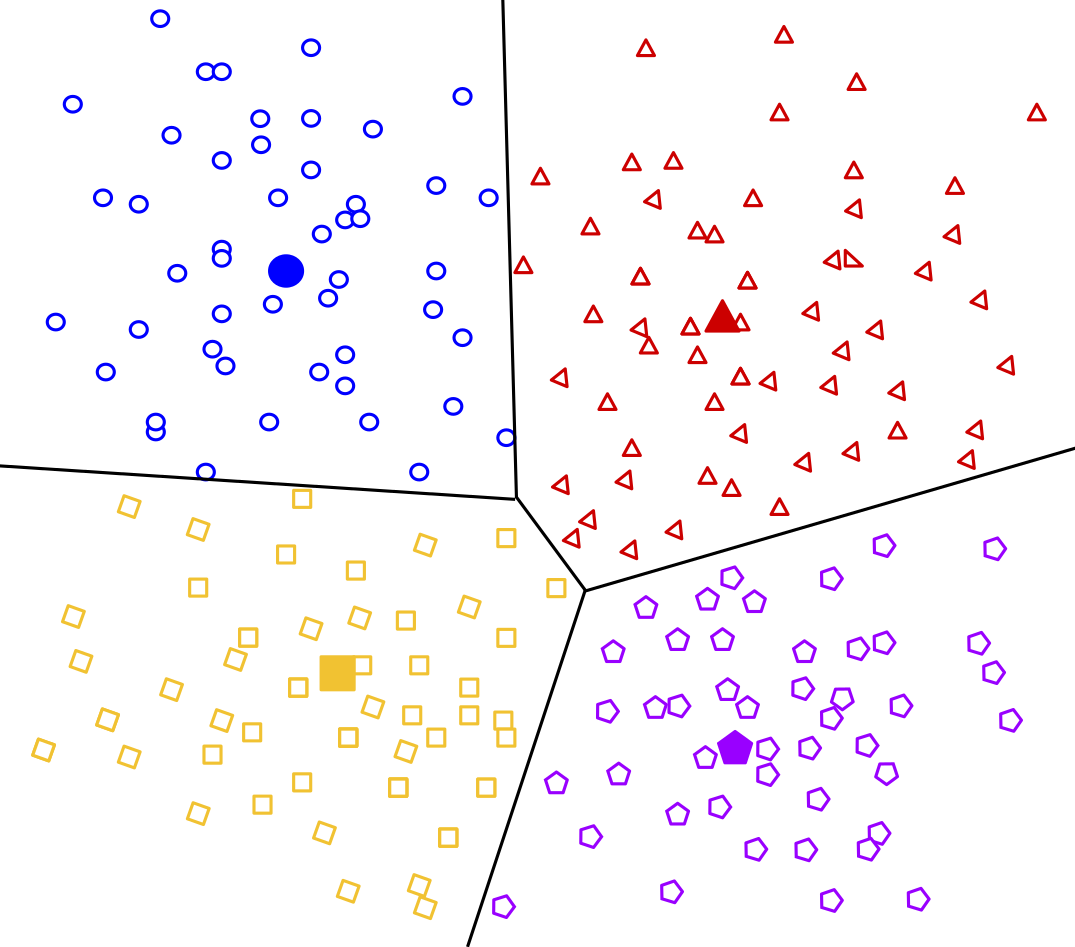
\includegraphics[scale=0.7]{centroid_clustering.png}
	\end{frame}

	\begin{frame}{Hierarchical Clustering}
		\center
		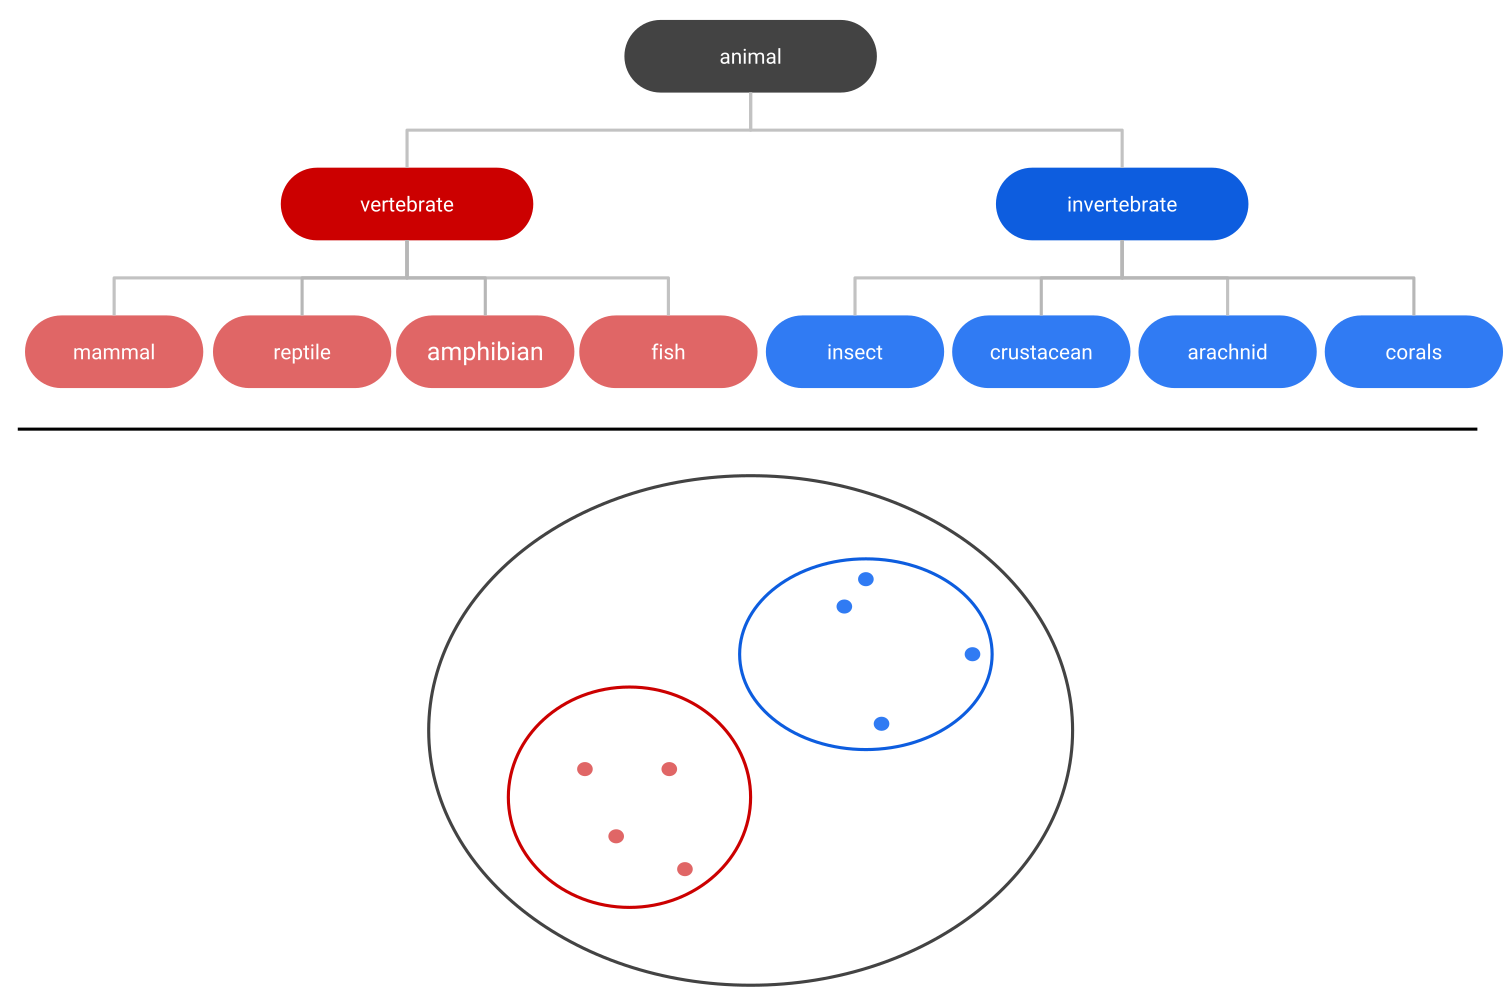
\includegraphics[scale=0.7]{hierarchical_clustering.png}
	\end{frame}

	\begin{frame}{Density-Based Clustering}
		\center
		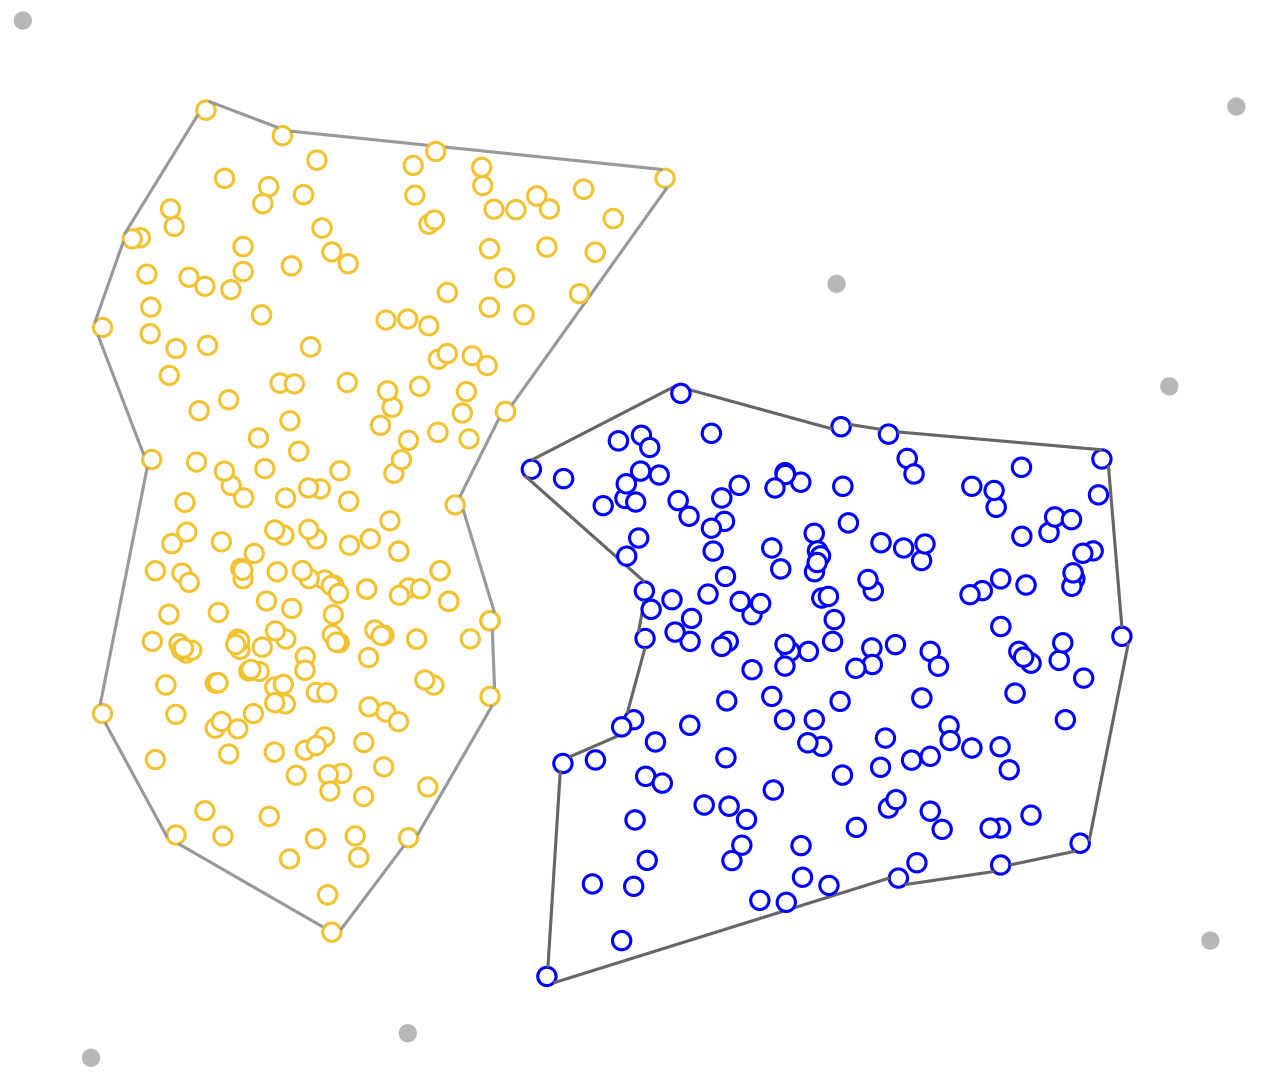
\includegraphics[scale=0.7]{density_clustering.png}
	\end{frame}

	\begin{frame}{Distribution-Based Clustering}
		\center
		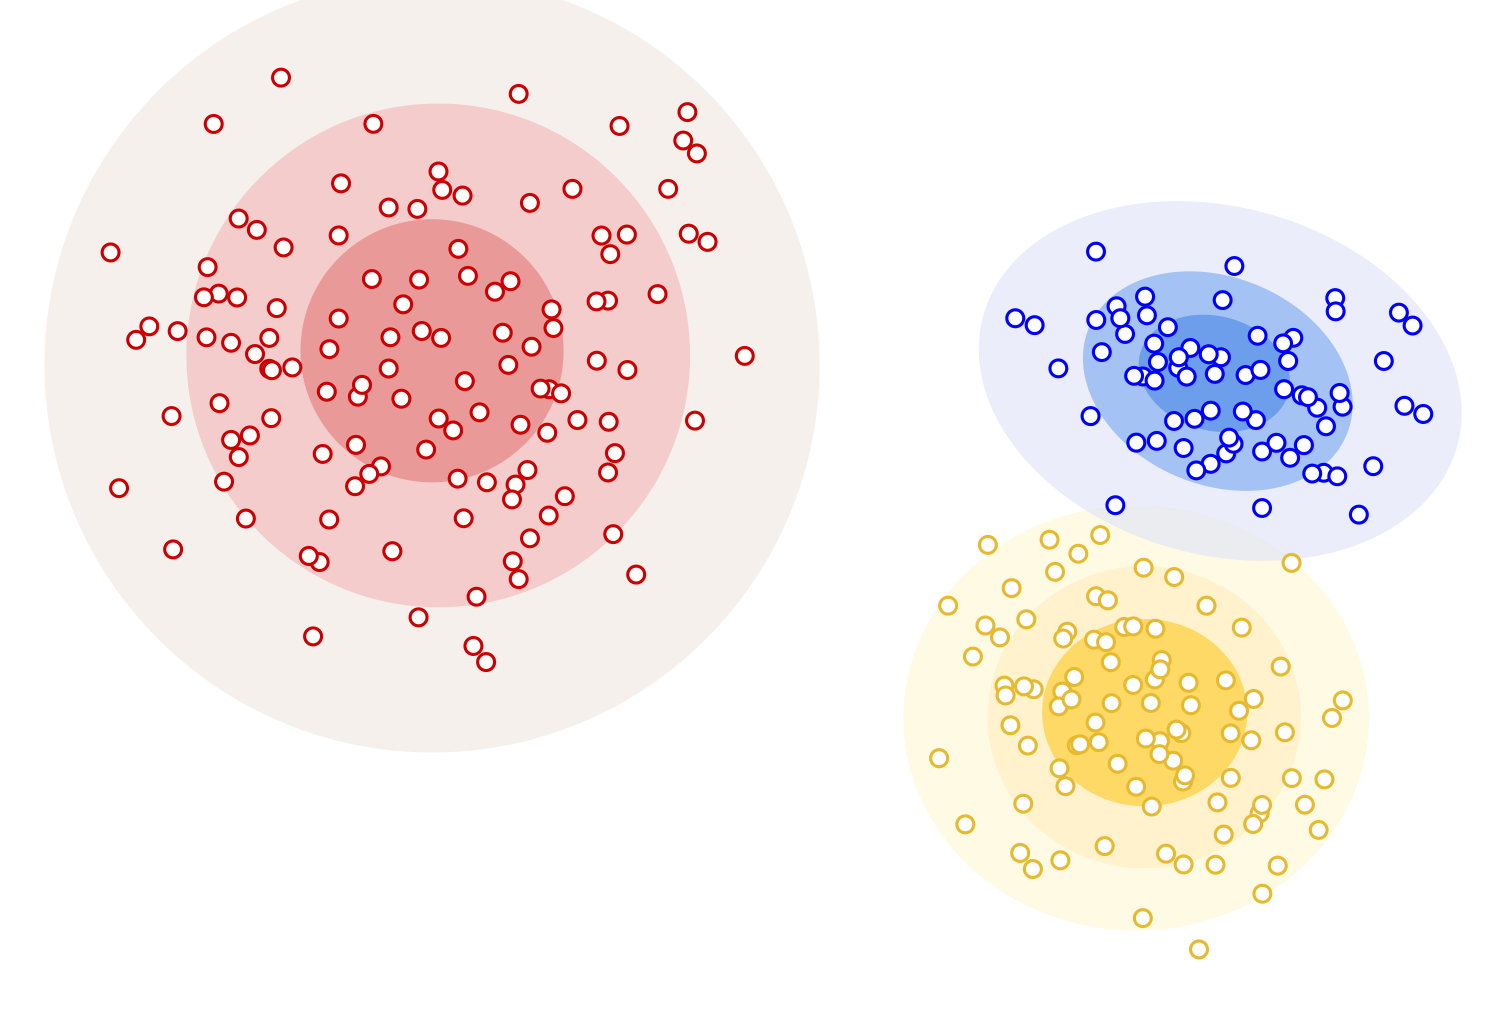
\includegraphics[scale=0.7]{distribution_clustering.png}
	\end{frame}
	
	\begin{frame}{Common Algorithms}
		\begin{itemize}
			\item K-Means
			\begin{itemize}
				\item minimizes the sum of squared distances from each point to its assigned centroid
				\pause
				\item \textit{requires the number of clusters to be specified}
				\pause
			\end{itemize}
			\item Hierarchical Clustering
			\pause
			\begin{itemize}
				\item Agglomerative: starts with each point as its own cluster, and merges the closest clusters
				\pause
				\item Divisive: starts with all points in one cluster, and repeatedly splits the cluster
				\pause
			\end{itemize}
			\item DBSCAN
			\begin{itemize}
				\item \textit{Density-Based Spatial Clustering of Applications with Noise}
				\pause
			\end{itemize}
			% \item HDBSCAN
			% \item Agglomerative Clustering
			\item Gaussian Mixture Models
			\begin{itemize}
				\item assumes that the data is generated from a mixture of several Gaussian distributions
			\end{itemize}
		\end{itemize}
	\end{frame}

	\section{HDBSCAN}
	\begin{frame}
		\begin{itemize}
			\item HDBSCAN stands for ``Hierarchical Density-Based Spatial Clustering of Applications with Noise''
			\pause
			\item It was introduced in 2015, by Campello, Moulavi, and Zimek \cite{hdbscan_paper}, for automatic clustering of n-dimensional data sets.
			\pause
			\item It uses a ``mutual reachability distance'', and identifies clusters by iteratively merging or splitting groups of data points.
		\end{itemize}
	\end{frame}

	\begin{frame}{$\core_k$}
		\begin{definition}\label{def:corek}
			Given some $k \in \mathbb{Z}^+$, for a data point $x$, the $\core_k (x)$ is the distance to the $k$-nearest neighbor of $x$.
		\end{definition}
		Note that this definition depends on which distance we are using.
		Usually we will use the $\ell^2$ norm.

		If the language seems strange, it is inspired by the HDBSCAN algorithm itself.
	\end{frame}

	\begin{frame}{$\core_k$ Illustration}
		\center
		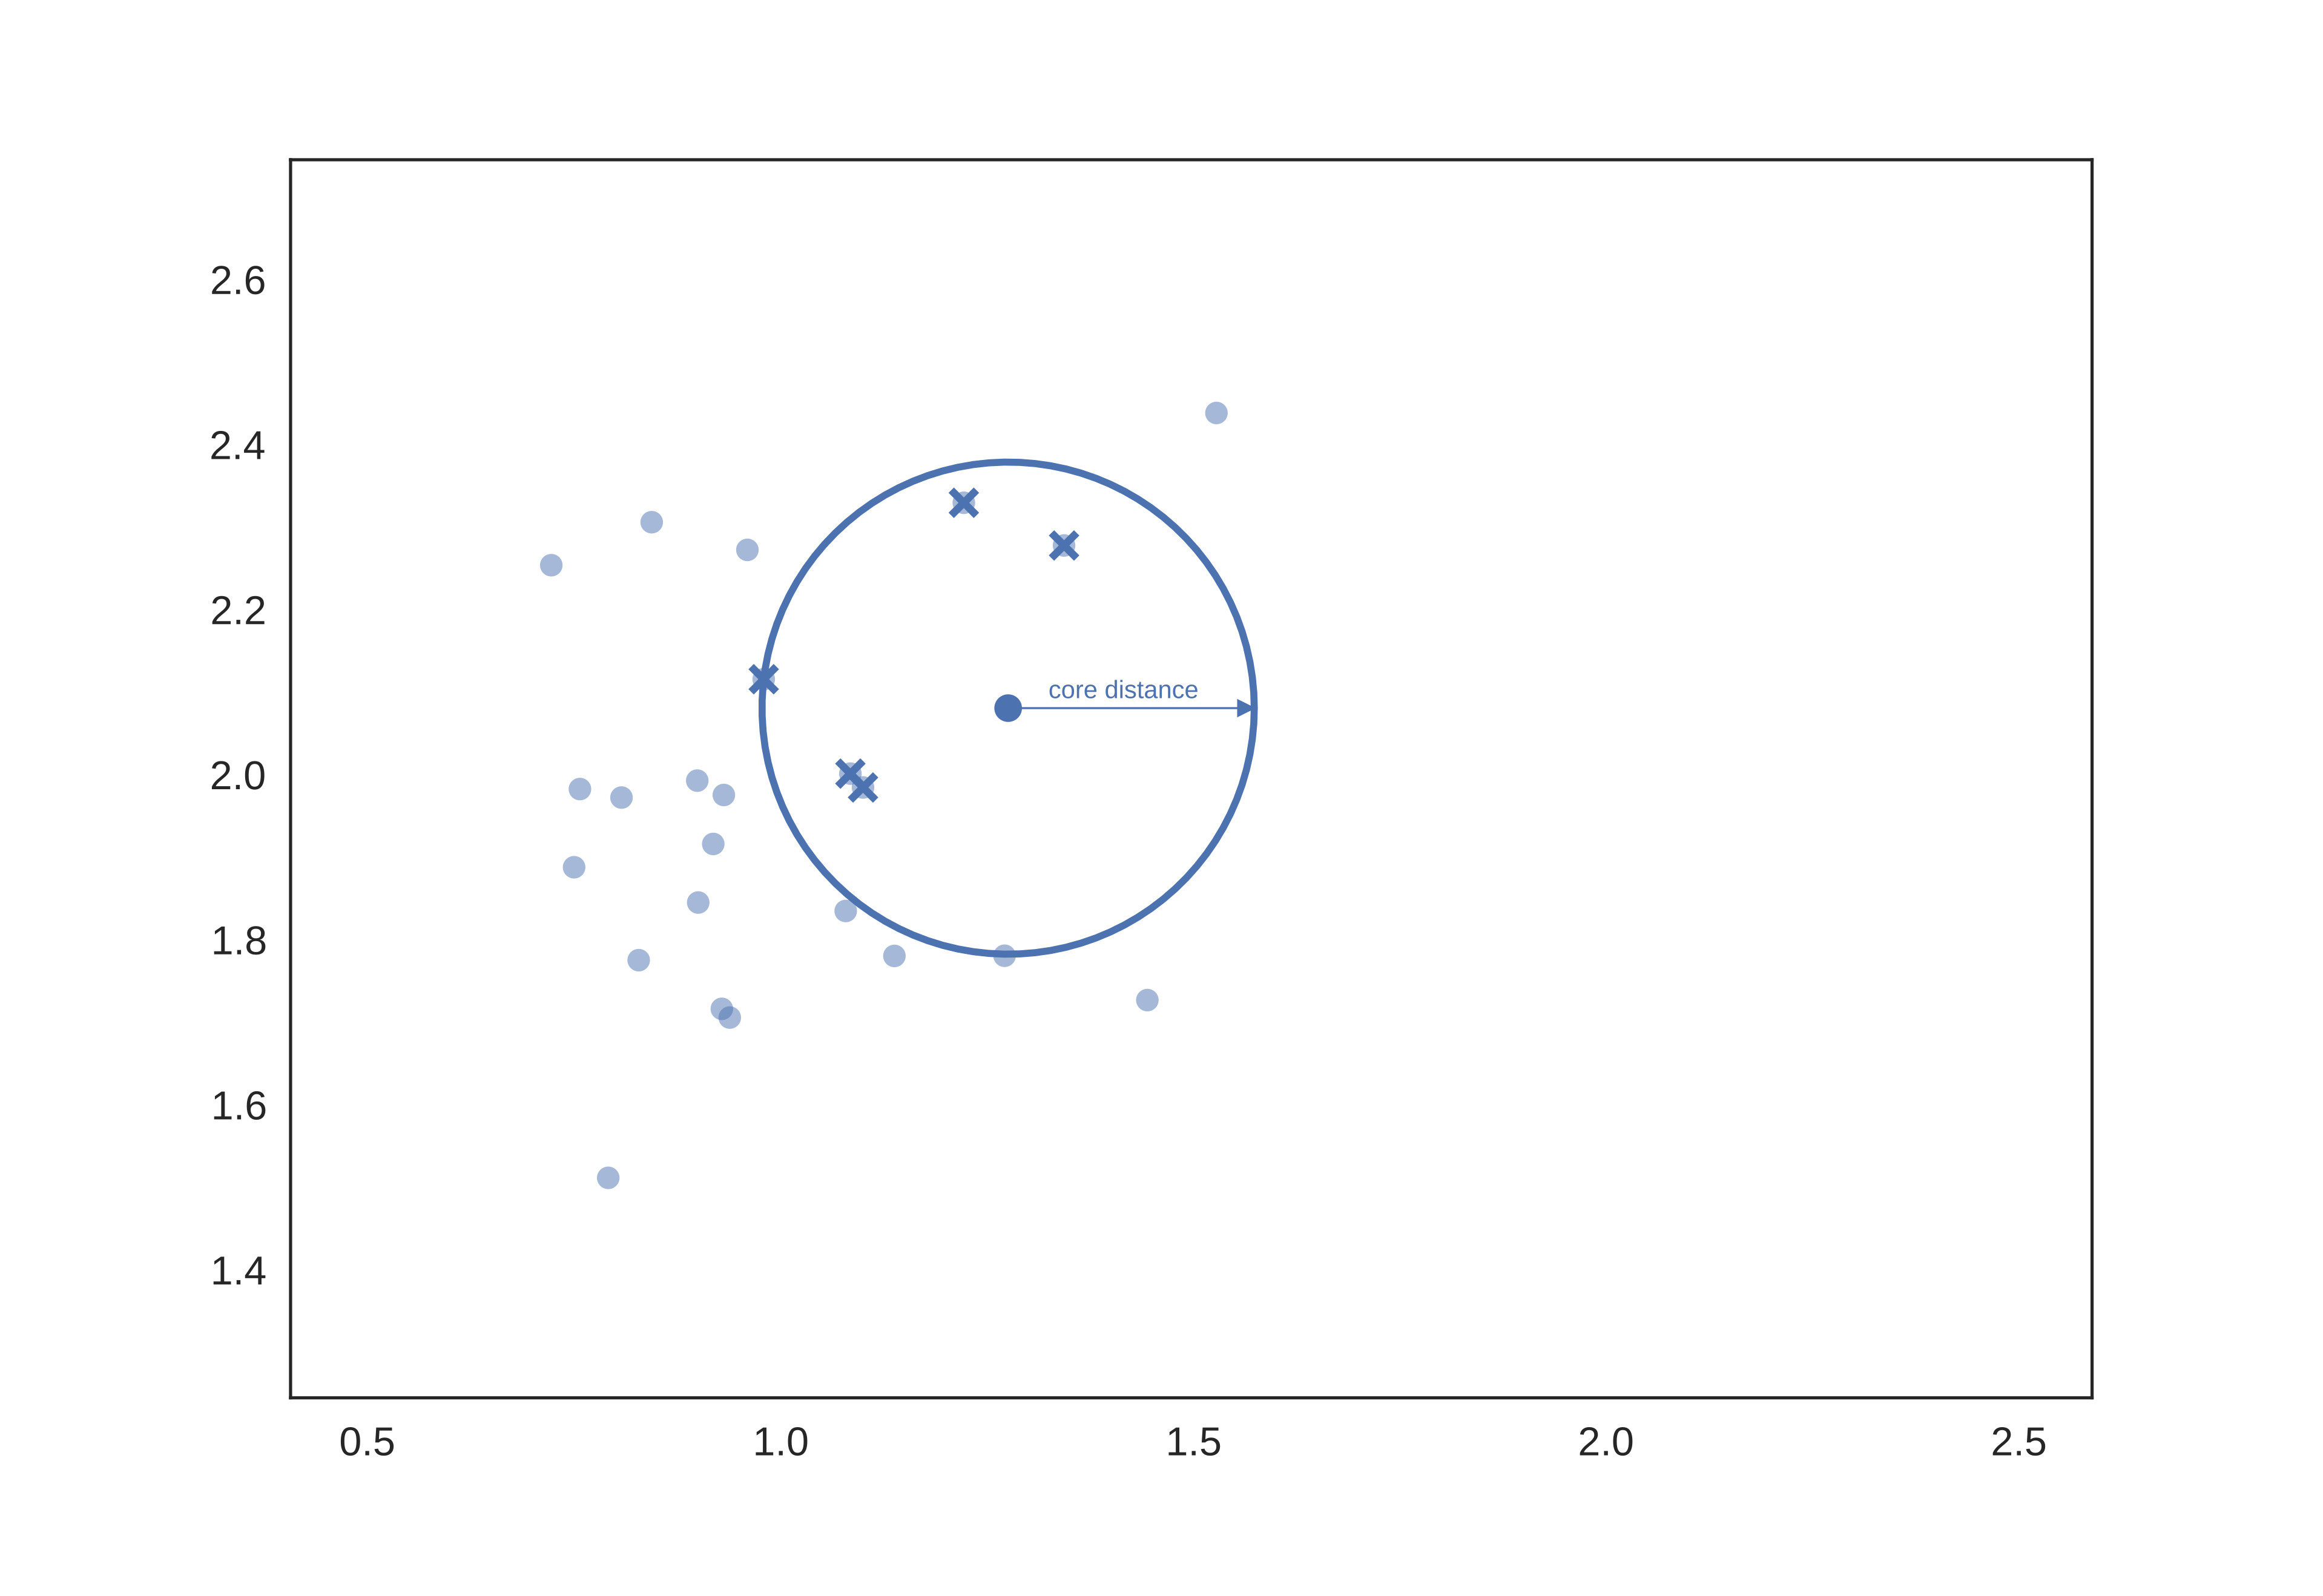
\includegraphics[scale=0.29]{core_example1.png}
	\end{frame}

	\begin{frame}{$\core_k$ Illustration}
		\center
		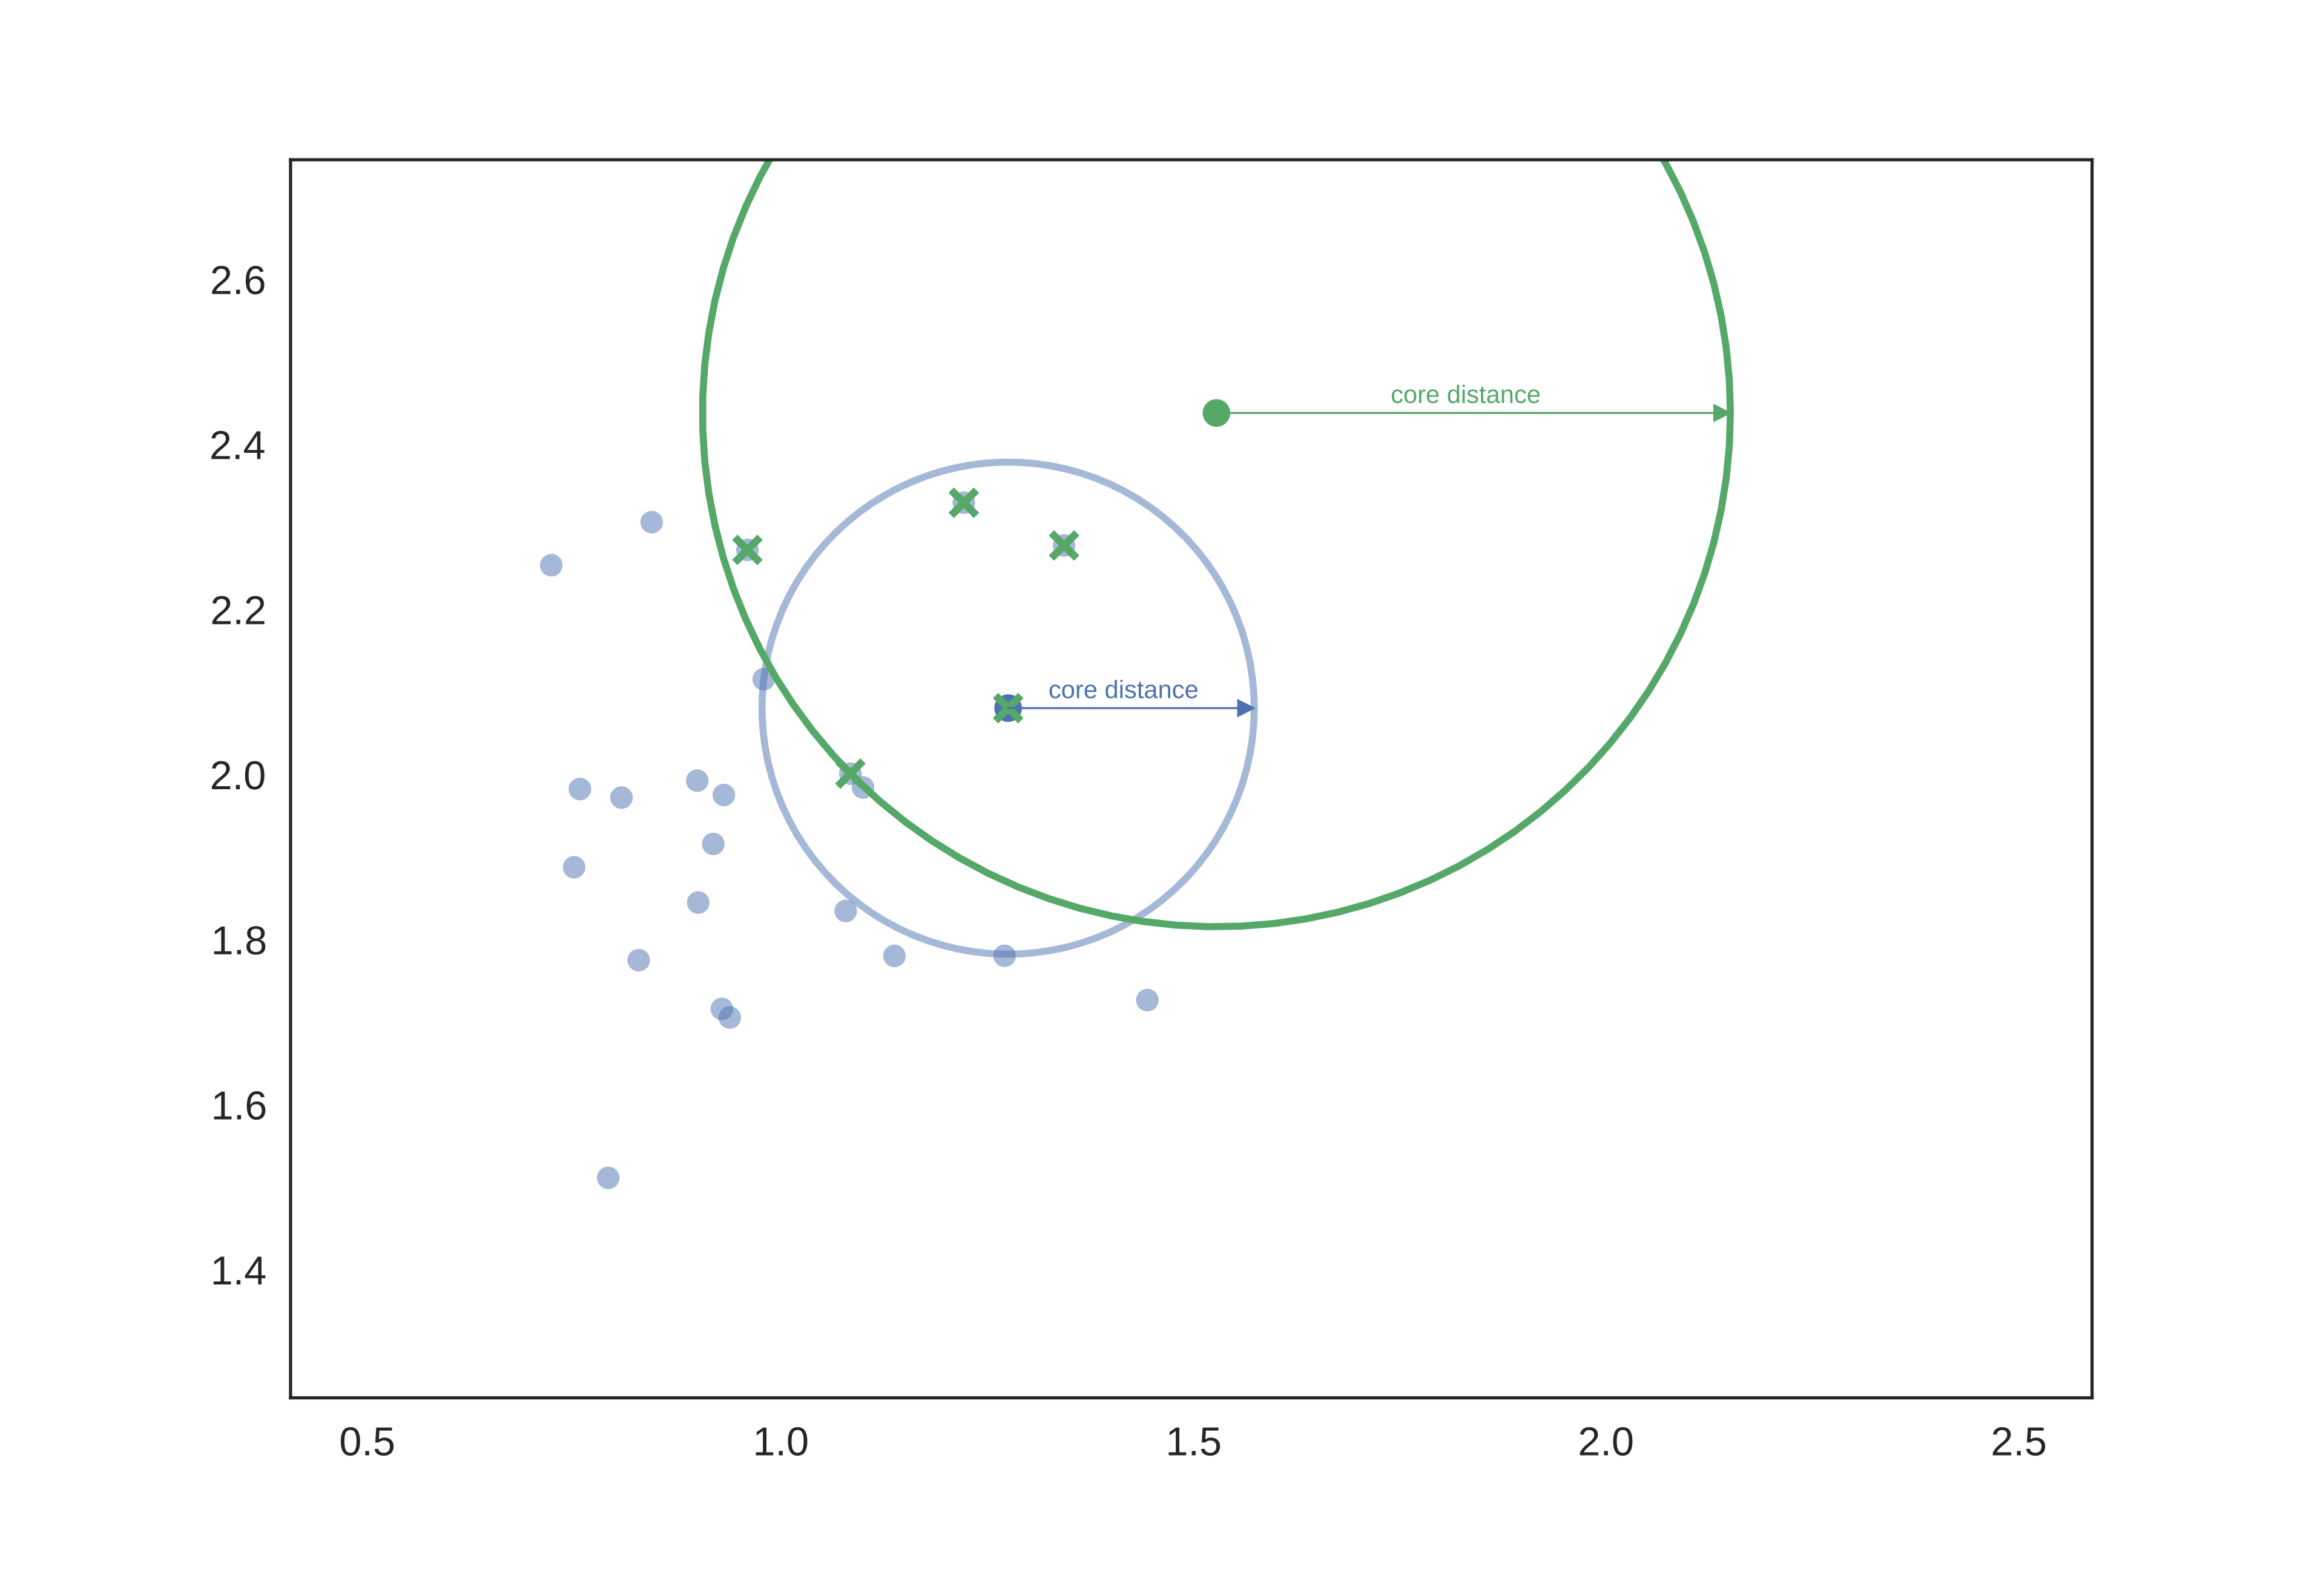
\includegraphics[scale=0.29]{core_example2.png}
	\end{frame}

	\begin{frame}{$\core_k$ Illustration}
		\center
		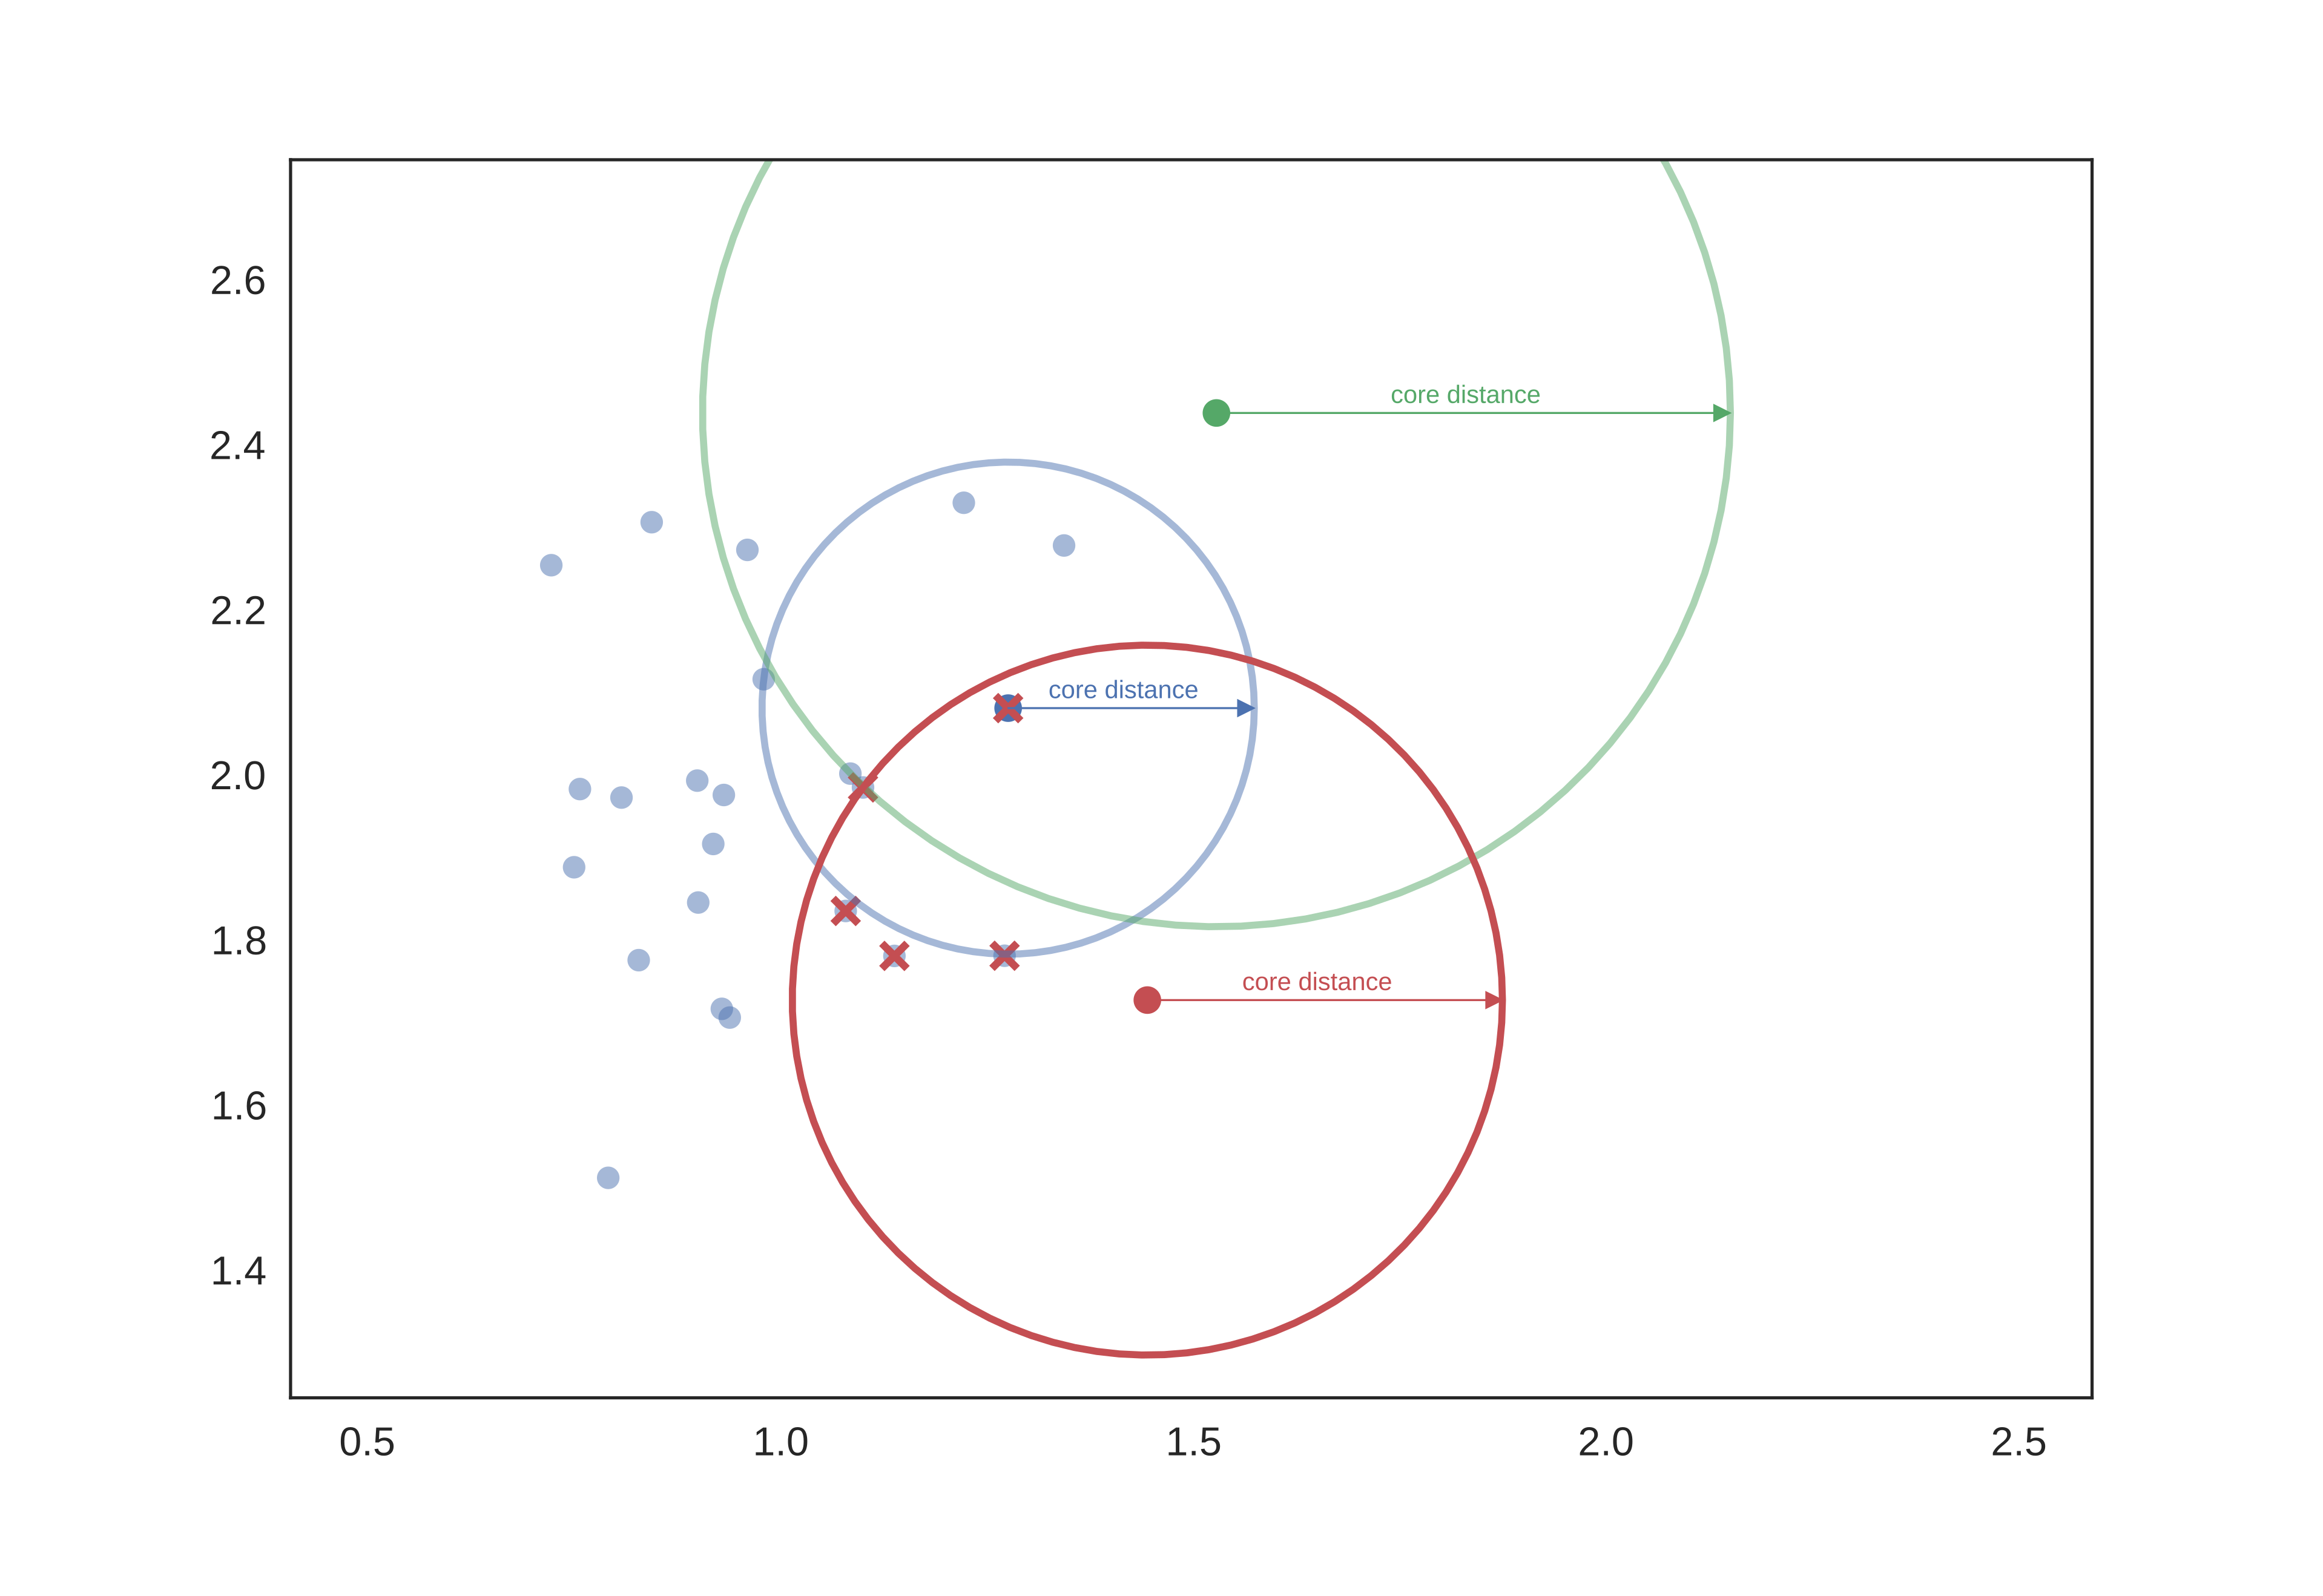
\includegraphics[scale=0.29]{core_example3.png}
	\end{frame}

	\begin{frame}{Mutual Reachability Distance}
		\begin{definition}\label{def:mrd}
			The \textbf{mutual reachability distance} of two data points $x$ and $y$, written $\mrd(x, y)$, with a paramater $k \in \mathbb{Z}^+$ and a metric $\dist$, is
			$$
			\max
			\begin{cases}
				\dist(x, y): \text{ Distance between } x \text{ and } y \\
				\core_k(x): \text{ Distance to $k$-nearest neighbor of } x \\
				\core_k(y): \text{ Distance to $k$-nearest neighbor of } y \\
			\end{cases}
			$$
			where ``distance'' refers to the standard $\ell^2$ norm of $x - y$, or euclidian distance (For our purposes).
		\end{definition}
		Note: The $k$-nearest neighbor is the $k$th closest point \textit{not counting the point itself}.
		Undefined if there are $k$ or less total data points.
	\end{frame}
	
	\begin{frame}{$\core_k$ Illustration}
		\center
		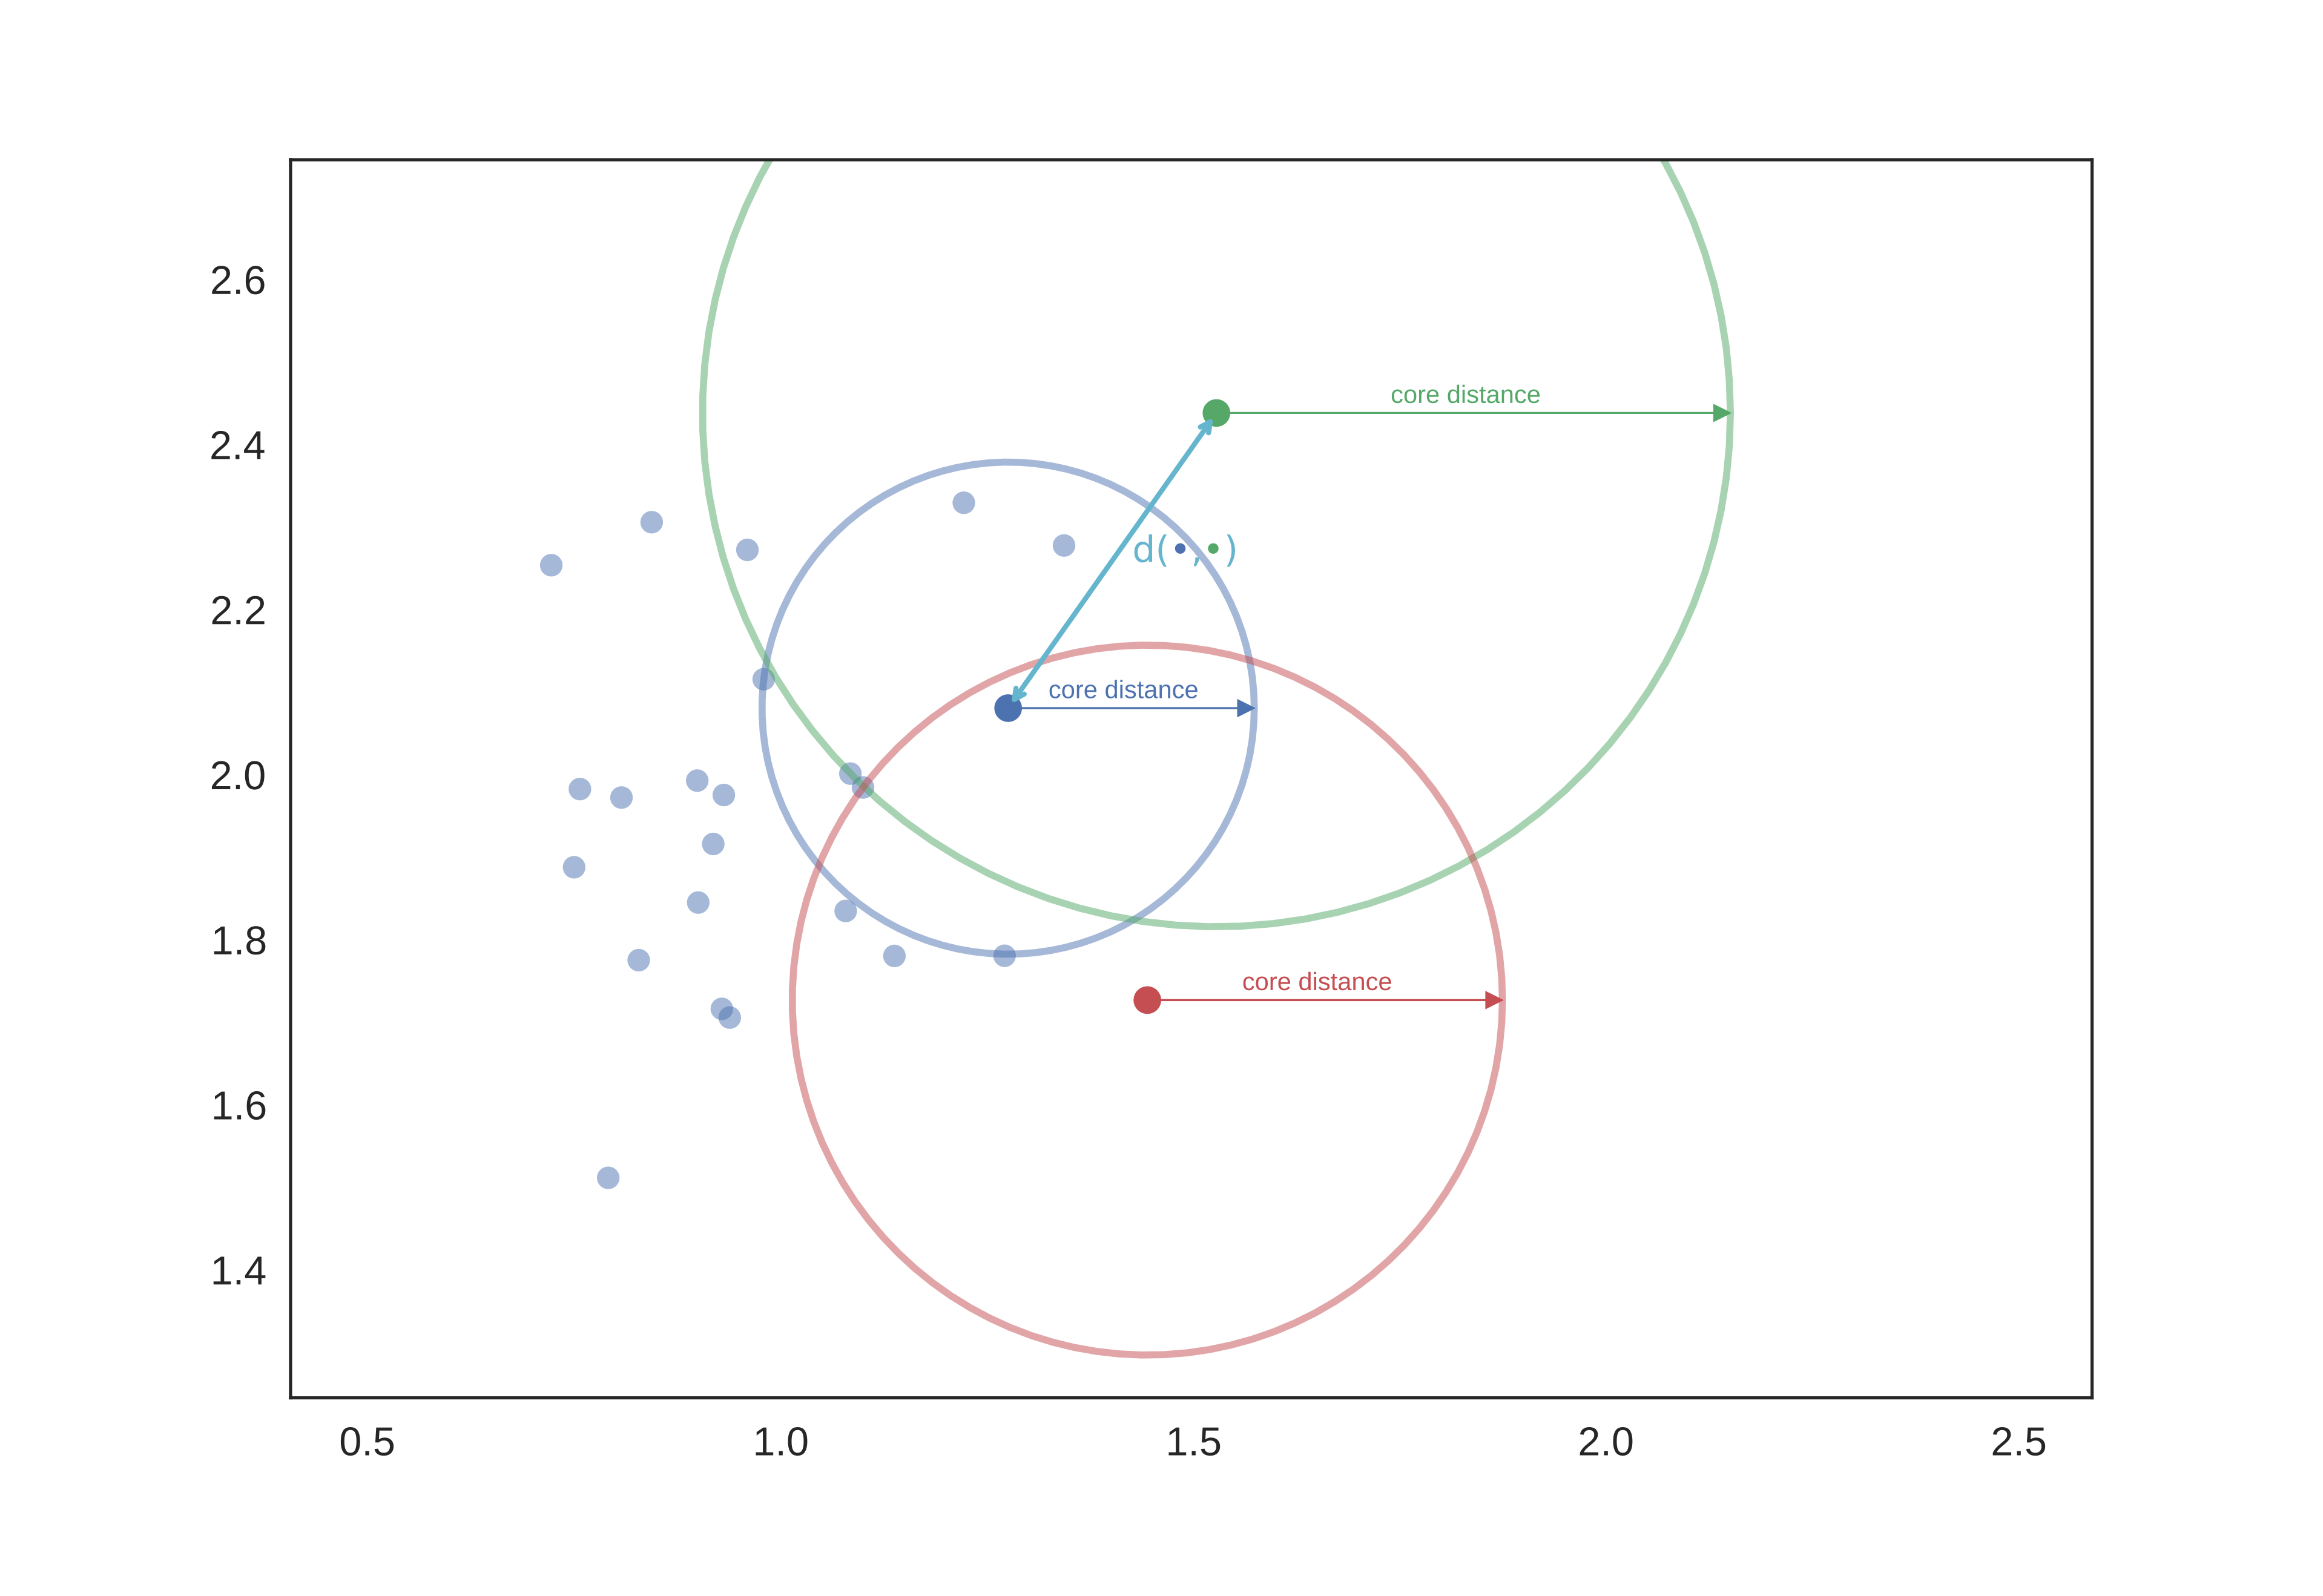
\includegraphics[scale=0.29]{core_example4.png}
	\end{frame}

	\begin{frame}{$\core_k$ Illustration}
		\center
		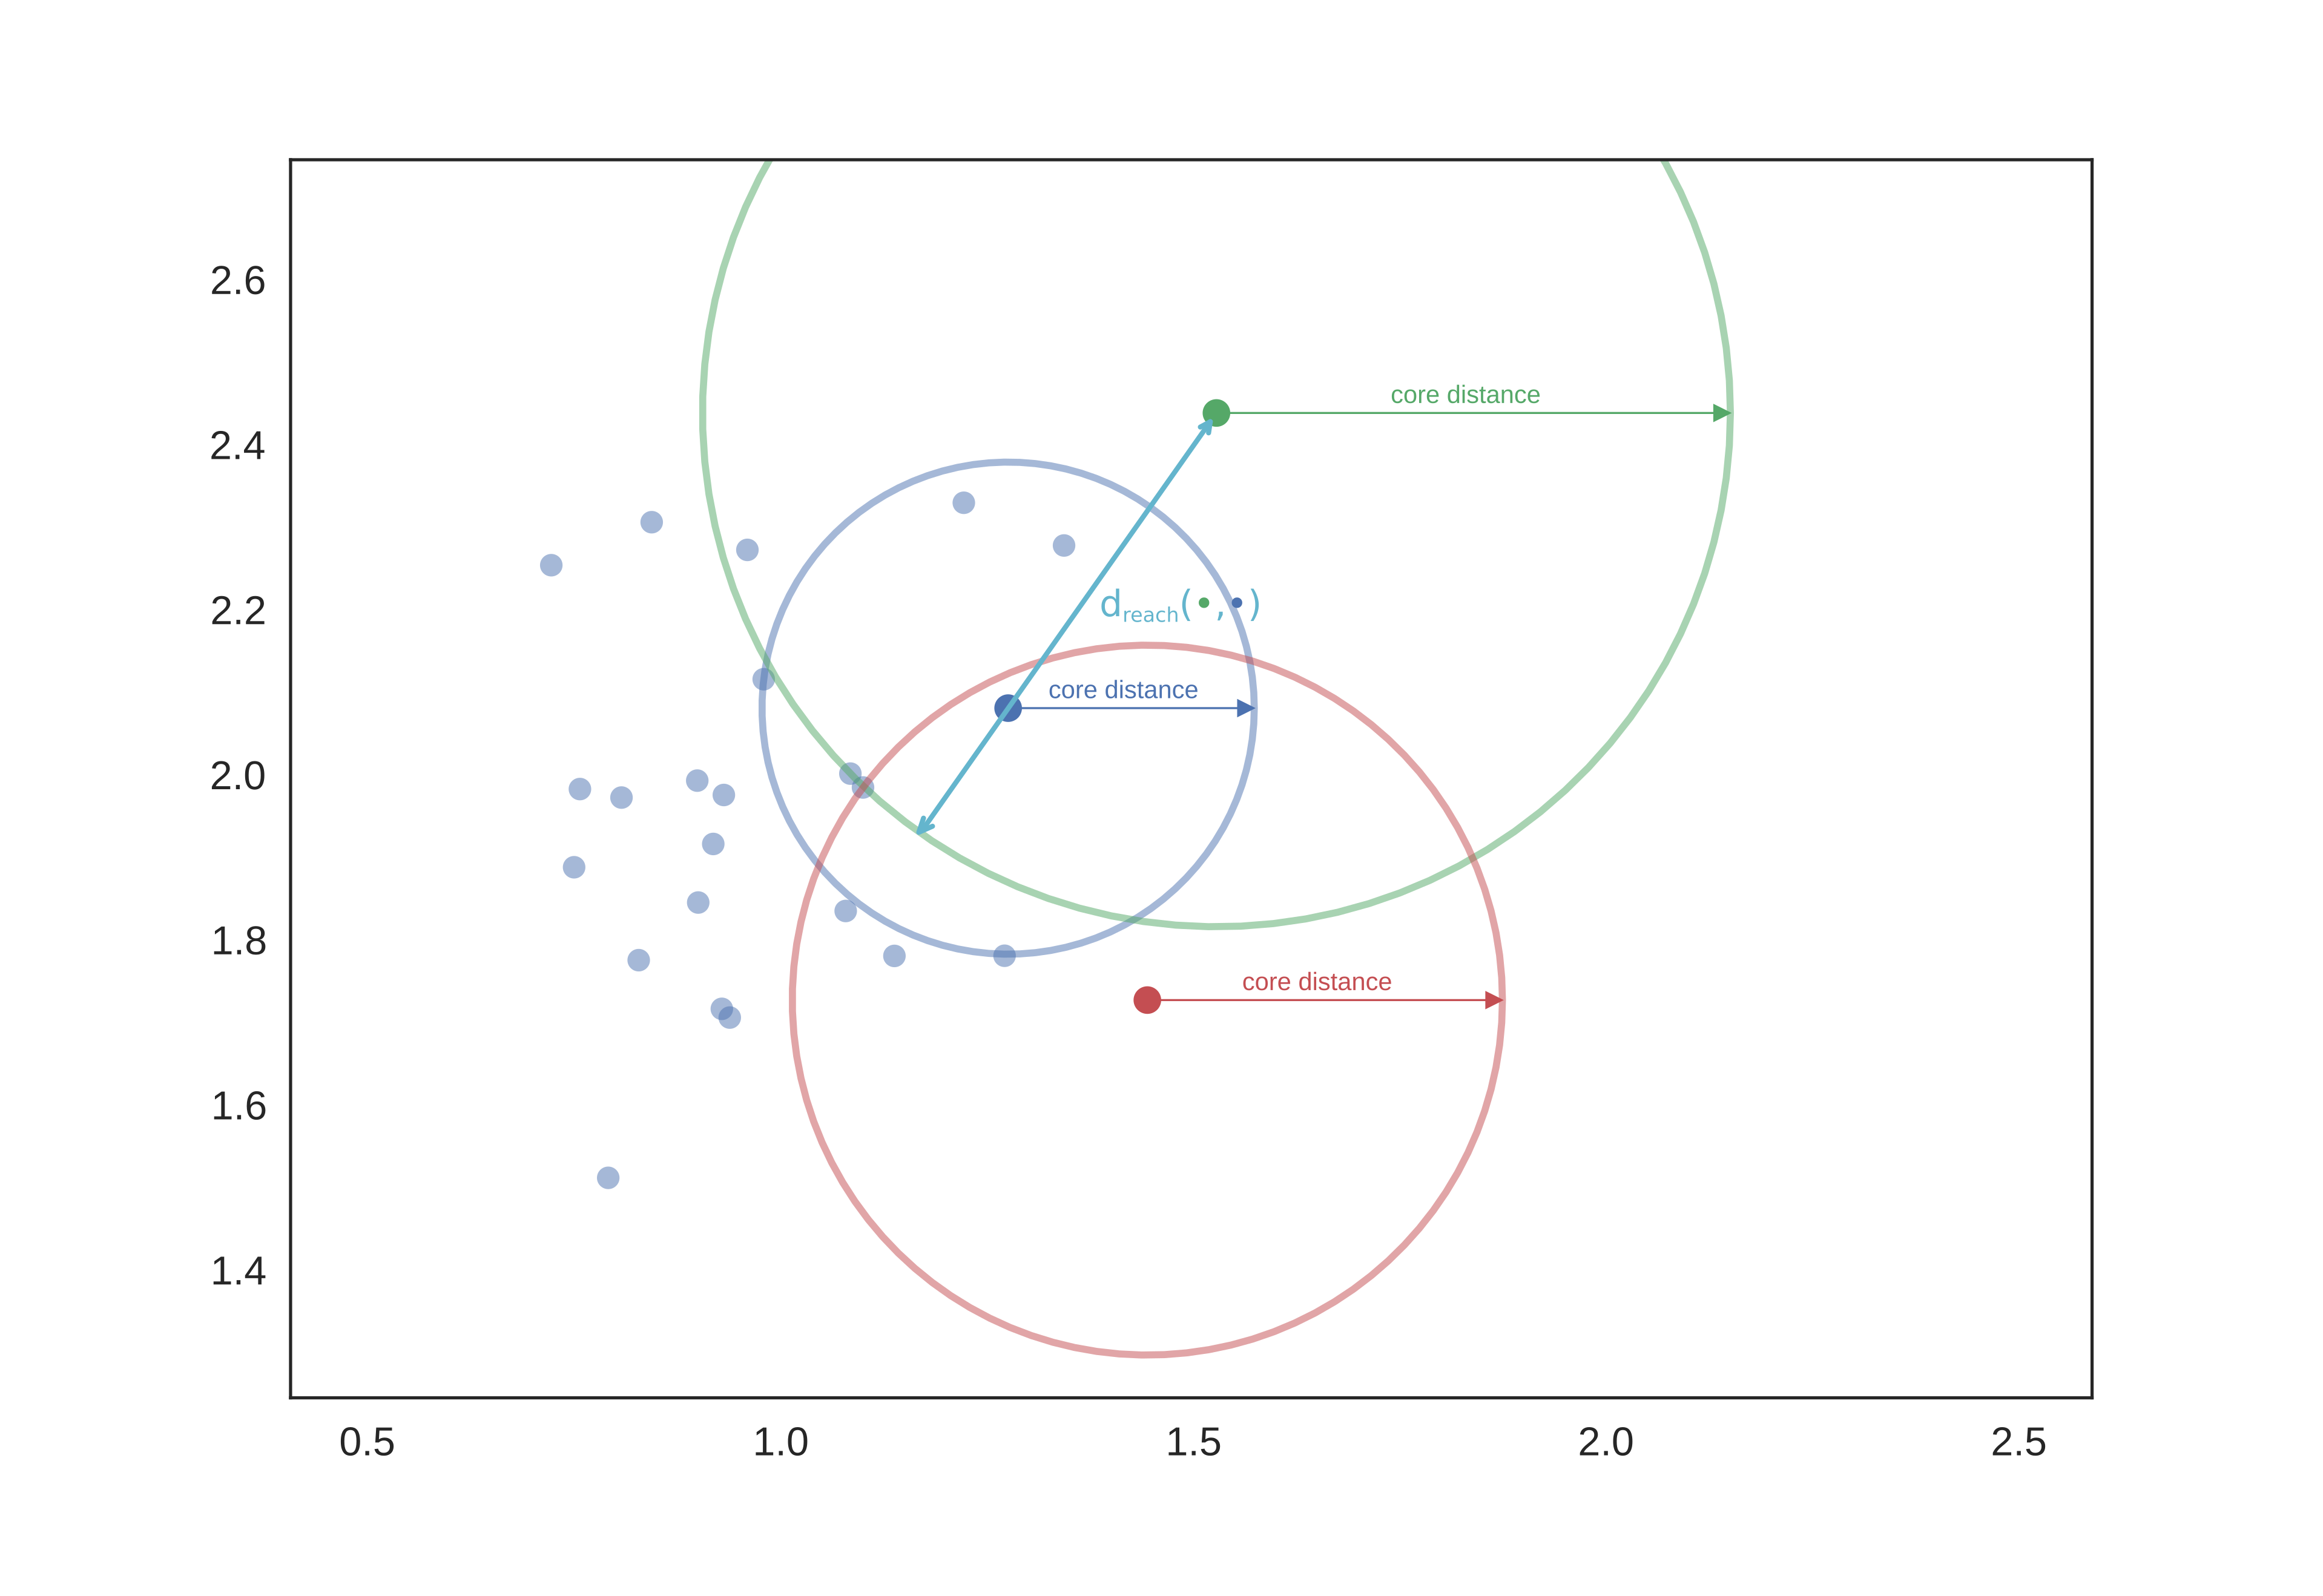
\includegraphics[scale=0.29]{core_example5.png}
	\end{frame}

	\begin{frame}{$\core_k$ Illustration}
		\center
		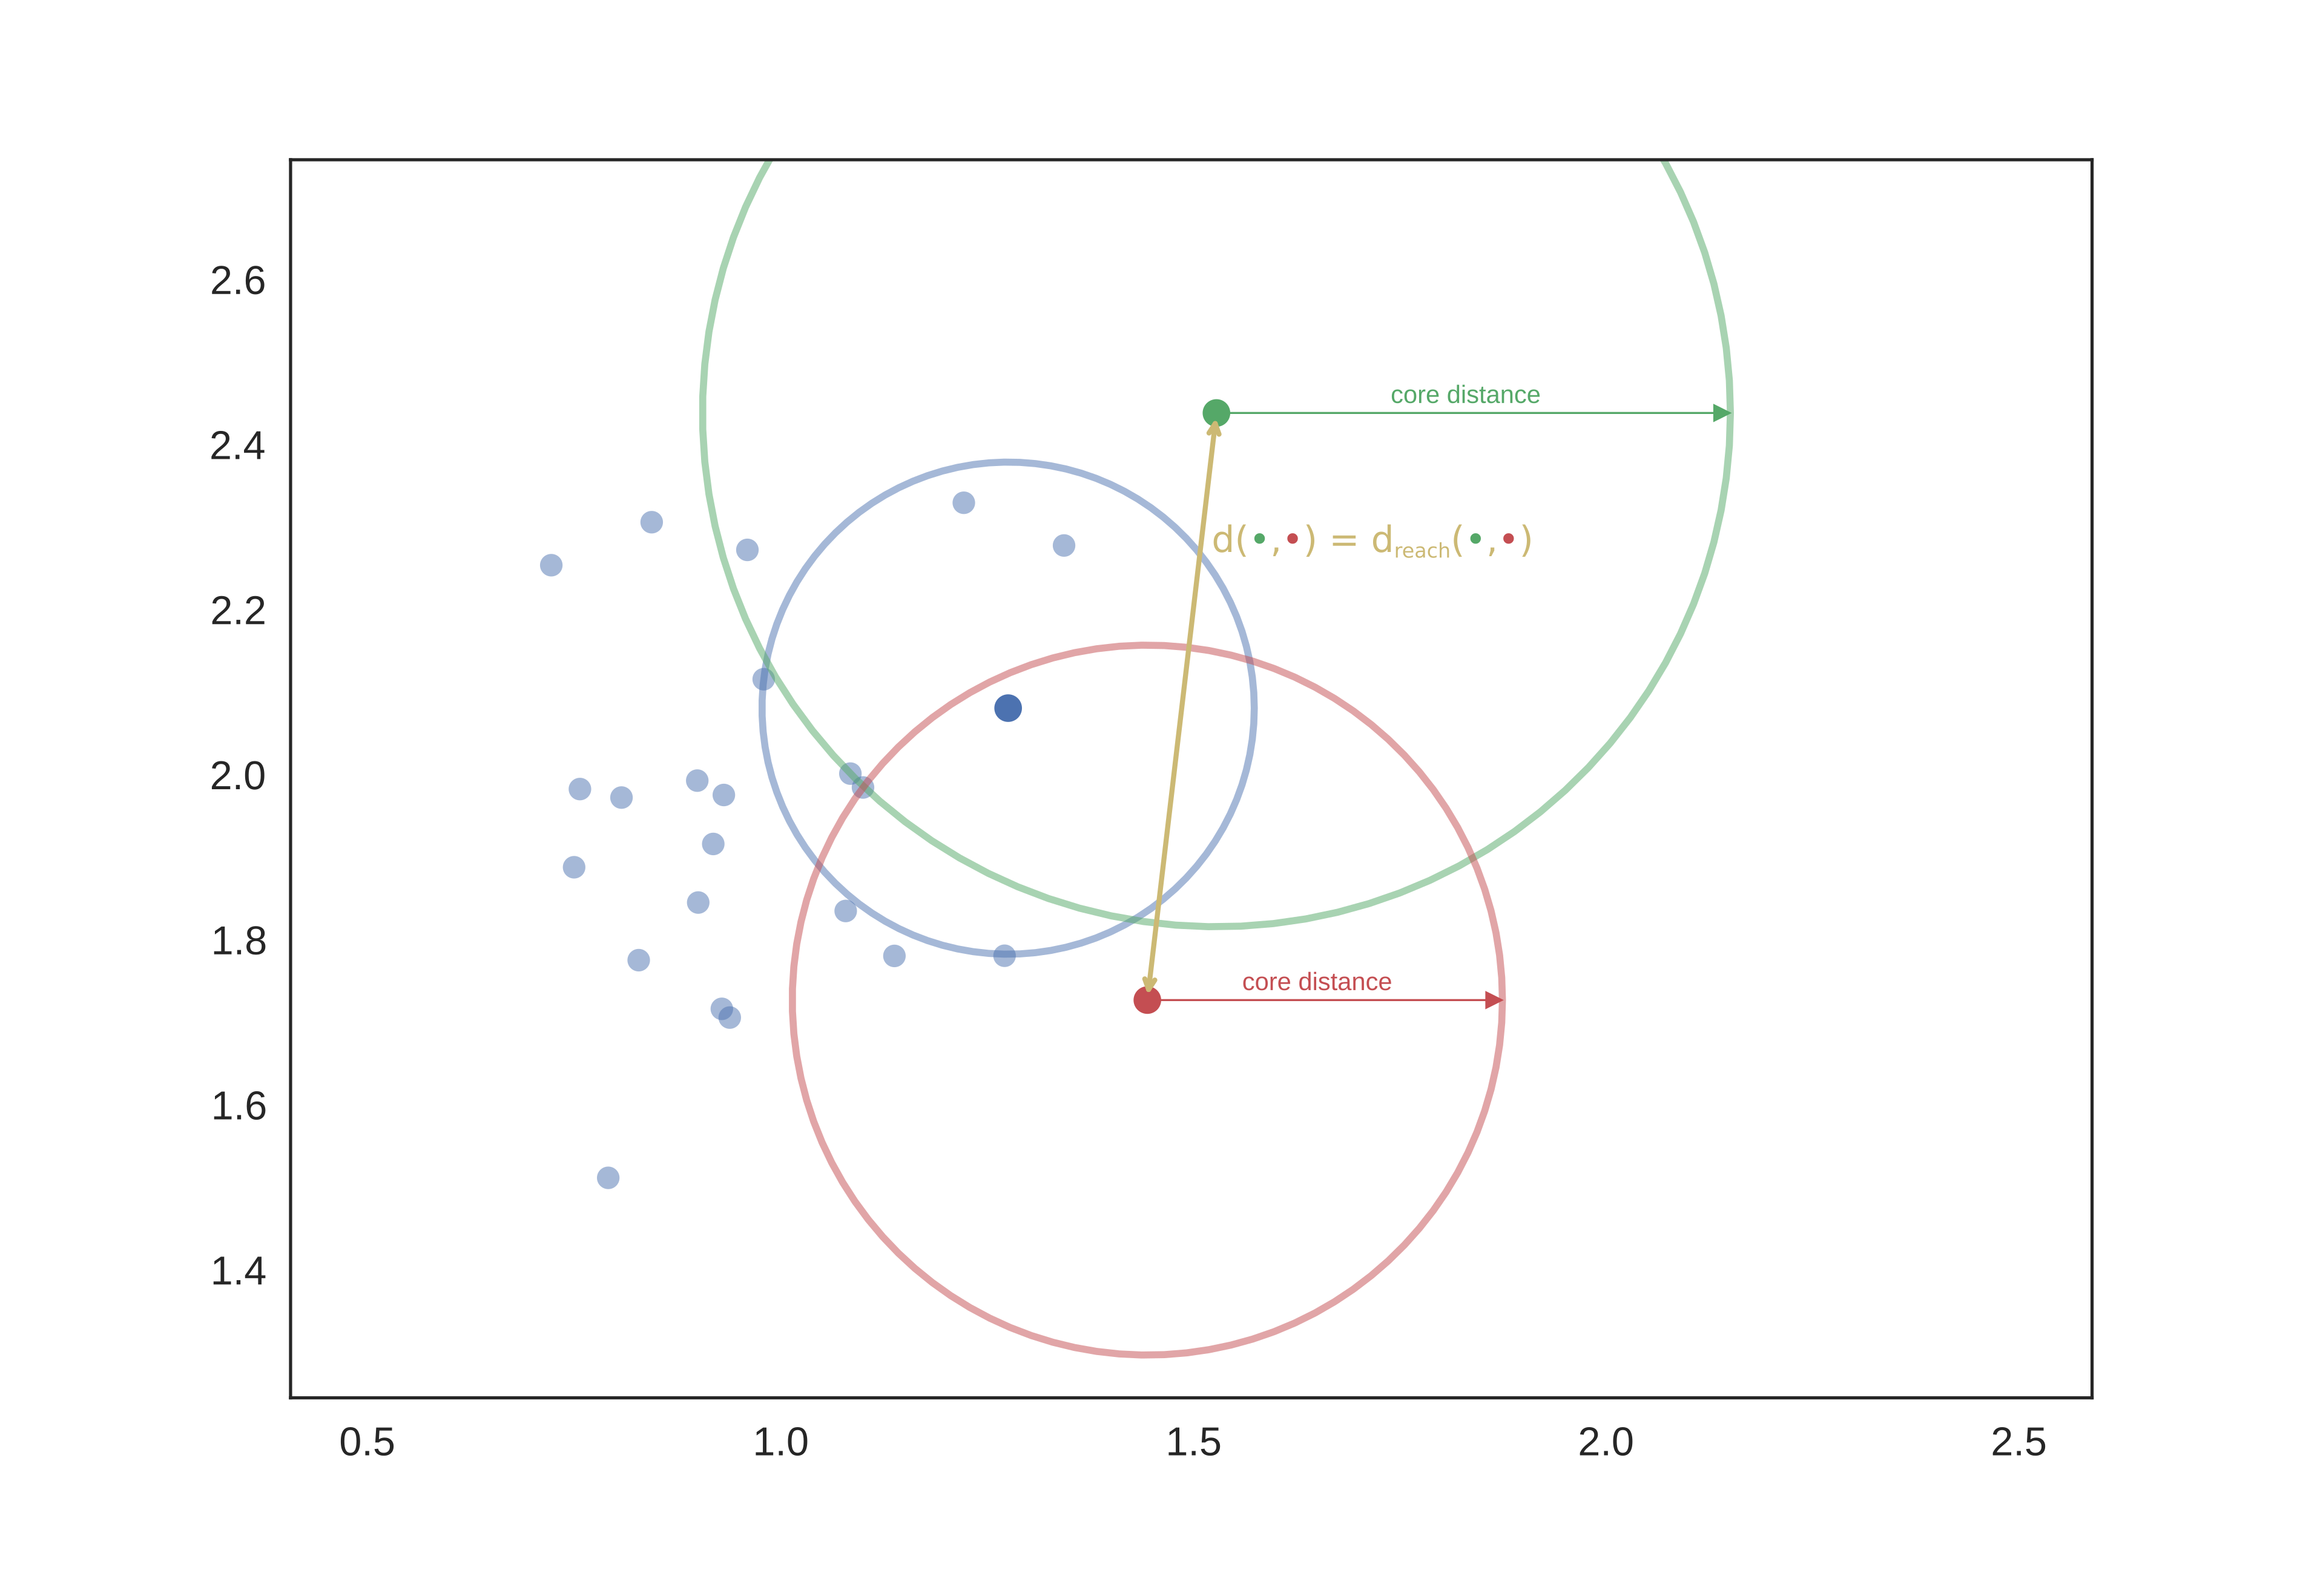
\includegraphics[scale=0.29]{core_example6.png}
	\end{frame}

	\begin{frame}{HDBSCAN}
		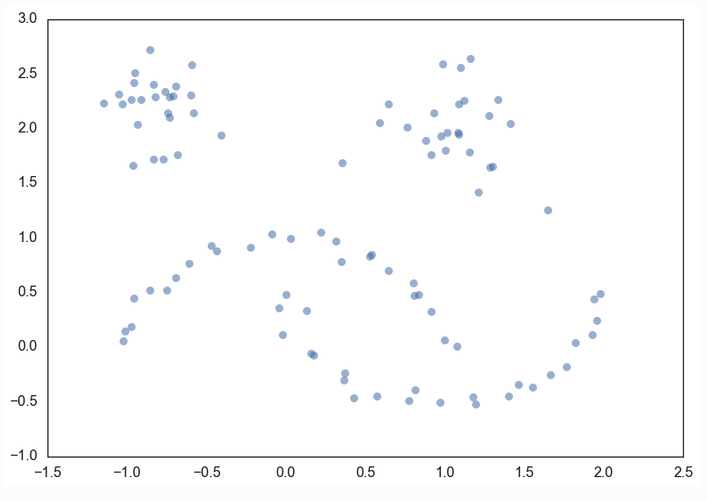
\includegraphics[scale=0.19]{from_tutorial/scatterplot.png}
		\pause
		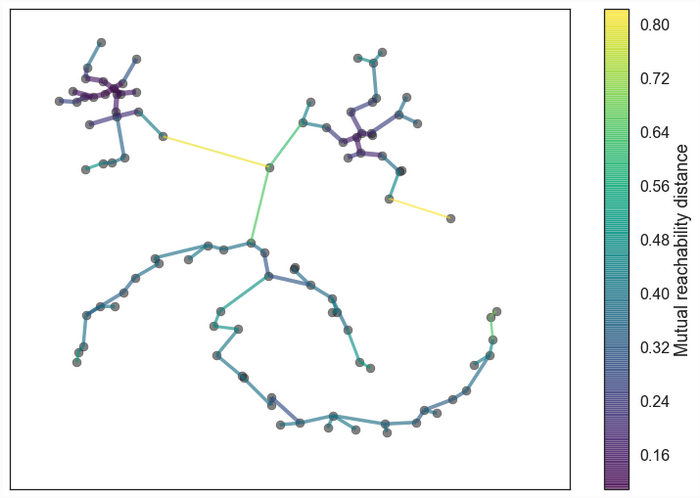
\includegraphics[scale=0.19]{from_tutorial/mst.png}
		\pause
		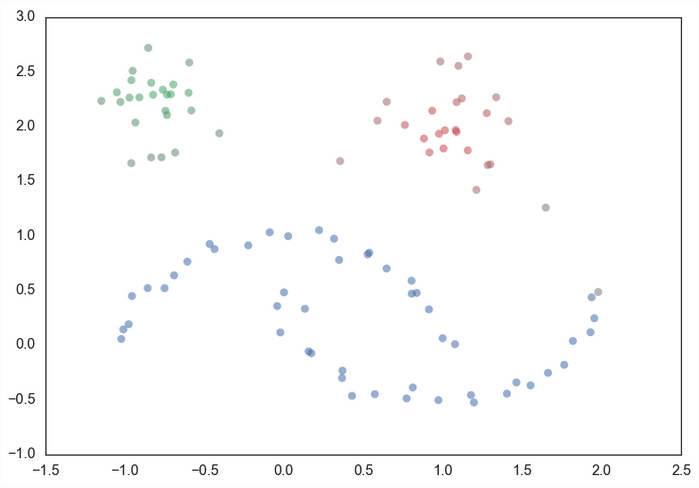
\includegraphics[scale=0.19]{from_tutorial/clusters.png}
	\end{frame}

	\begin{frame}{Example HDBSCAN Run}
		\center
		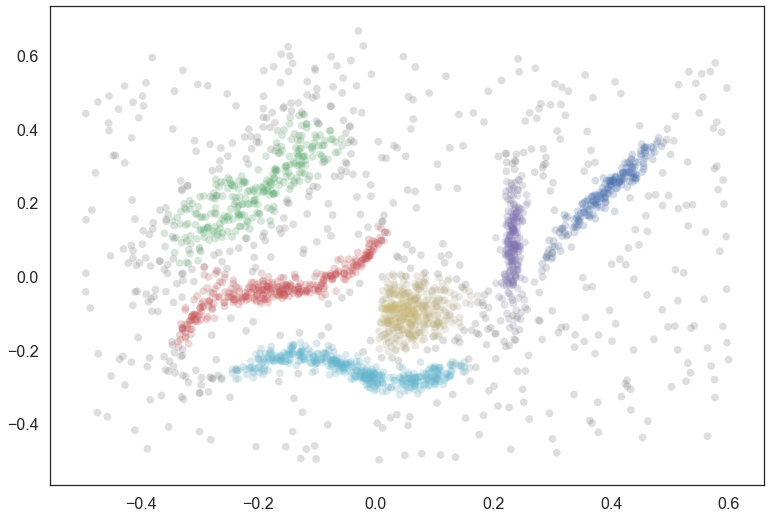
\includegraphics[scale=0.34]{sample_hdbscan_run.png}
	\end{frame}

	\begin{frame}{Forty Random Points}
		\center
		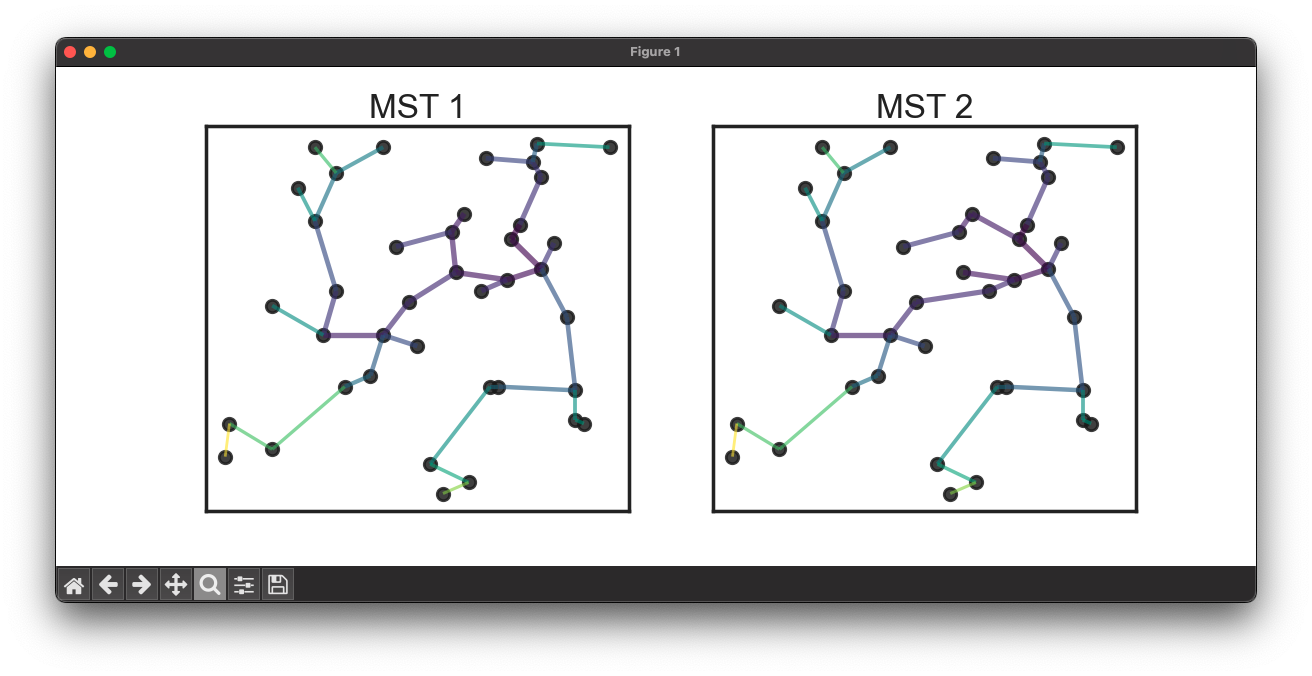
\includegraphics[scale=0.25]{forty_random.png}
	\end{frame}

	\begin{frame}{``Unreasonable Stability''}
		In \cite{blevins_presentation}, Dr. Blevins and her advisor Dr. Bridges of Oak Ridge National Labratory
		showed that distinct minimum spanning trees on the same data set give the same clusters.
		\center
		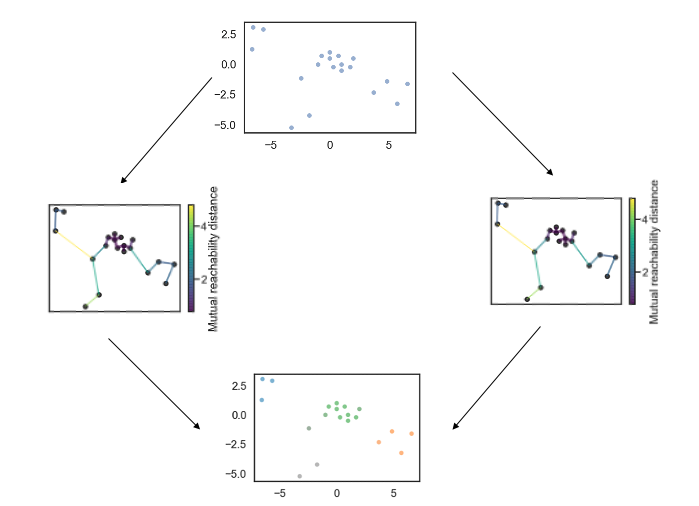
\includegraphics[scale=0.25]{stability.png}
	\end{frame}

	\begin{frame}{Goals}
		\begin{enumerate}
			\item Verify that it is possible to get different minimum spanning trees over the same data \label{goal1}
			\pause
			\item Test whether this can occur in real-world data (and get a rough sense of how often) \label{goal2}
			\pause
			\item Describe sufficient conditions for non-unique minimum spanning trees \label{goal3}
		\end{enumerate}
	\end{frame}

	\section{Python Testing}
	\begin{frame}{Base Case}
		\begin{example}
			Different orderings of the simple data set $[[0, 0], [0, 1], [1, 1], [1, 0]]$ give different minimum spanning trees
		\end{example}
		\center
		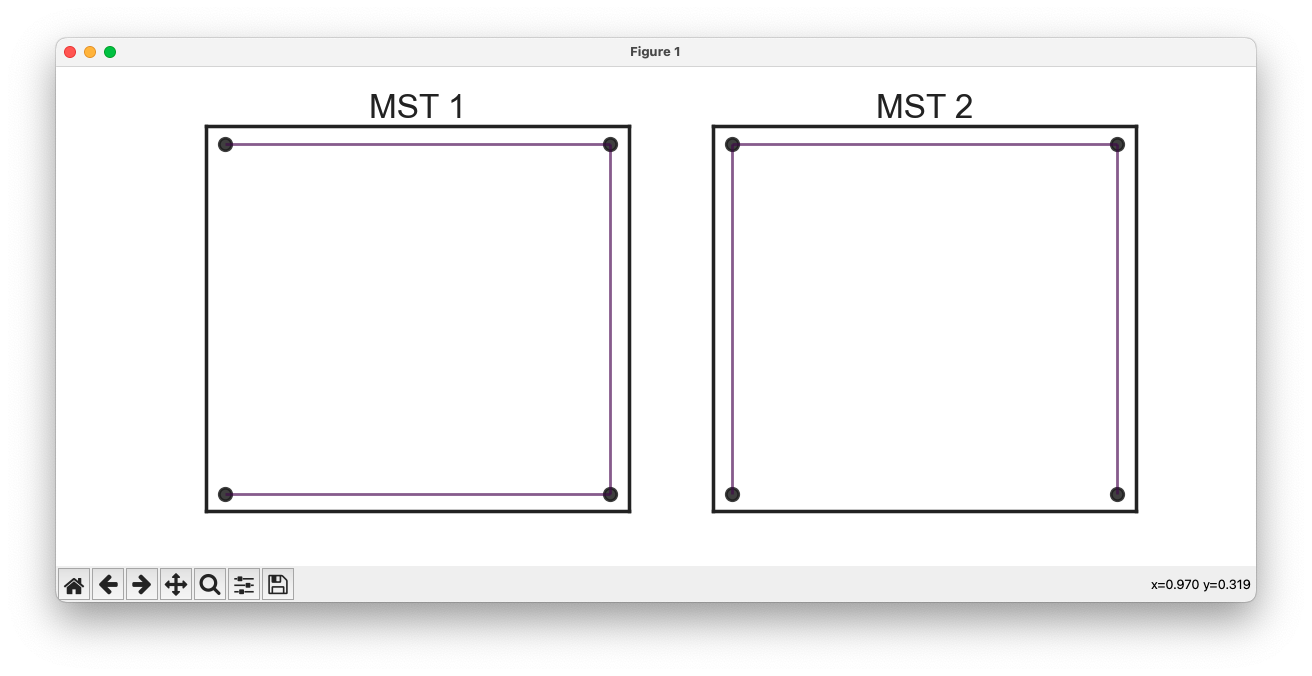
\includegraphics[scale=0.2]{base_case.png}
	\end{frame}

	\begin{frame}{Iris}
		\begin{example}
			the Iris data set \cite{Unwin2021TheID} records information about various types of iris flowers.
		\end{example}
		\center
		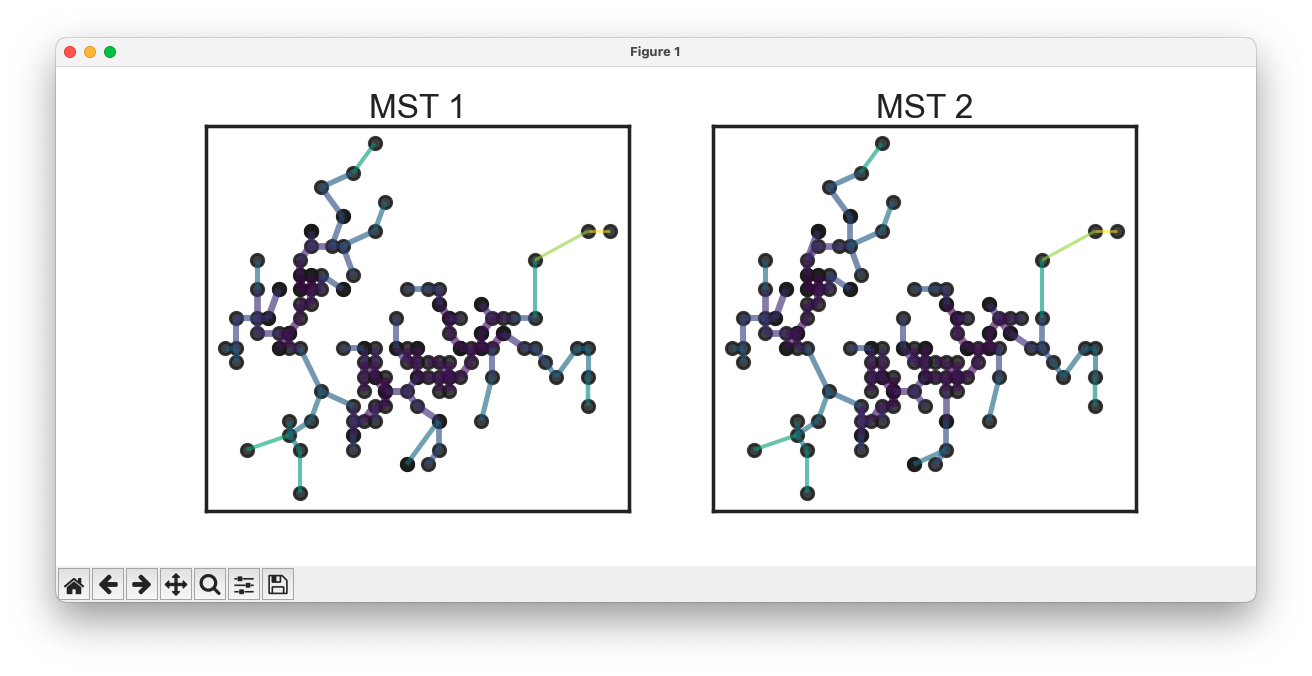
\includegraphics[scale=0.2]{iris2d.png}
	\end{frame}

	\begin{frame}{Iris Closeup}
		\begin{center}
			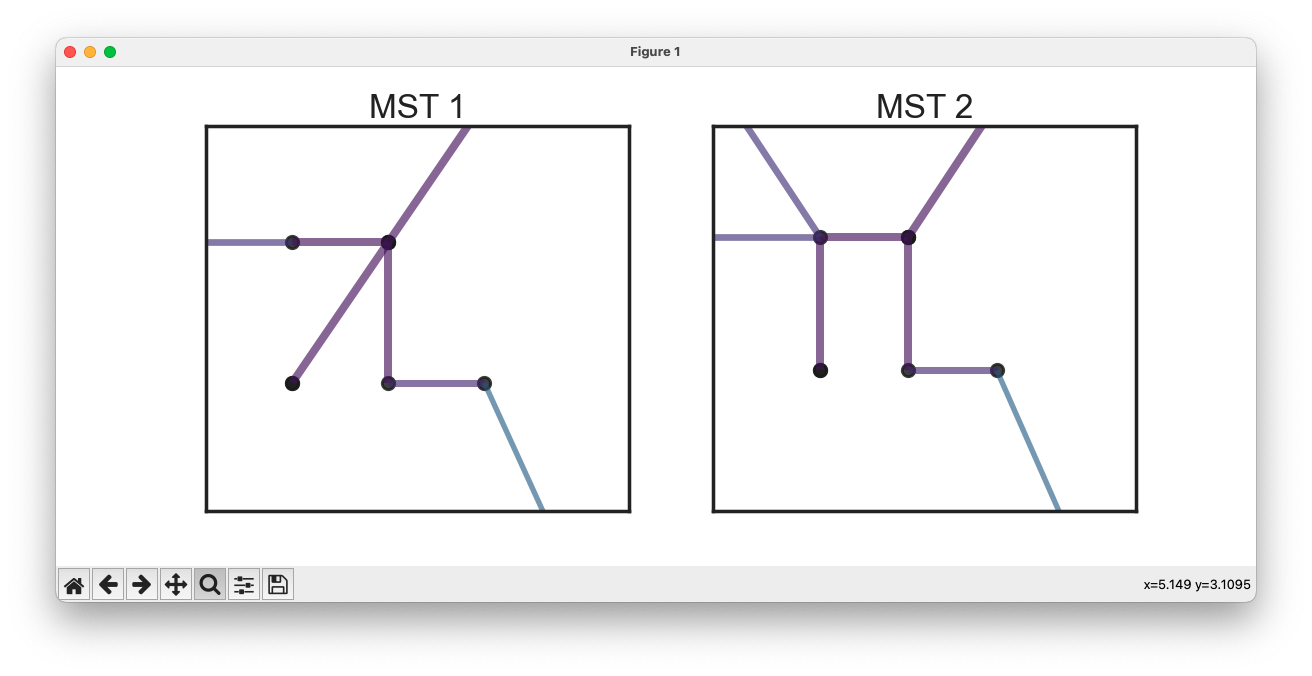
\includegraphics[scale=0.2]{iris2d_closeup.png} \\
		\end{center}
		Note: All graphs (except the first) are a two-dimensional projection of the higher-dimensional data sets, but the python script verifies that there are truly multiple trees in the native dimension.
	\end{frame}

	\begin{frame}{MNIST Closeup}
		\begin{example}
			MNIST is a massive data set of handwritten digits. We plotted the first 50.
		\end{example}
		\center
		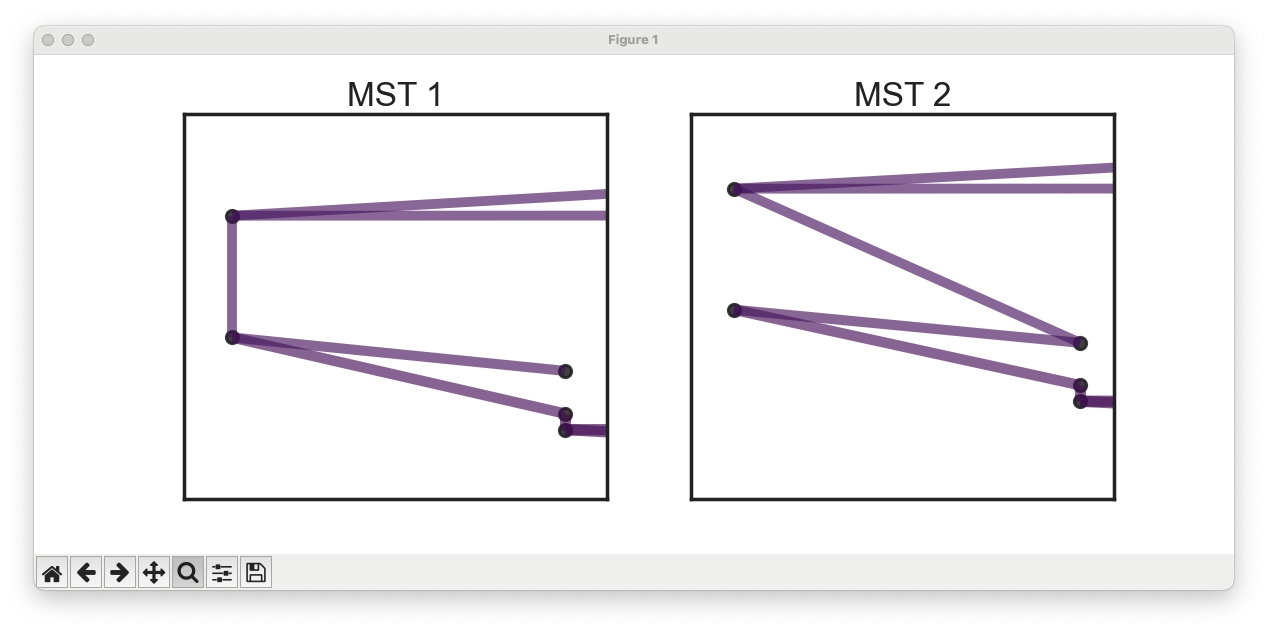
\includegraphics[scale=0.2]{mnist2d_closeup.png}
	\end{frame}
	
	\section{Two Dimensions}

	\begin{frame}{NEC\textit{k}Sc}
		\begin{definition}\label{def:necks}
			Let $X$, along with some distance definition $\dist$, be a finite metric space.
			And, with a paramater $k \in \mathbb{Z}^+$, define
			$$\epsilon = \min_{x \in X} \core_k(x) = \core_k(x_0) \text{ for some } x_0 \in X.$$
			Then $X$ is a `not-everywhere $\core_k$ sparse (closed)' (\textbf{NEC\textit{k}Sc}) metric space, if and only if
			$$\exists y, z \in \{ x \in X : 0 < \dist(x, x_0) \leq \epsilon \} \text{ with } y \neq z \text{ and } \dist(y, z) \leq \epsilon.$$
		\end{definition}
		In other words, a metric space is NEC\textit{k}Sc if there are two points in the $k$-nearest neighbors of $x_0$ that are also within $\epsilon$ of each other.
	\end{frame}

	\begin{frame}{Original NEC\textit{k}S Definition}
		Note: This is a tweaked version of a NEC\textit{k}S metric space.
		\center
		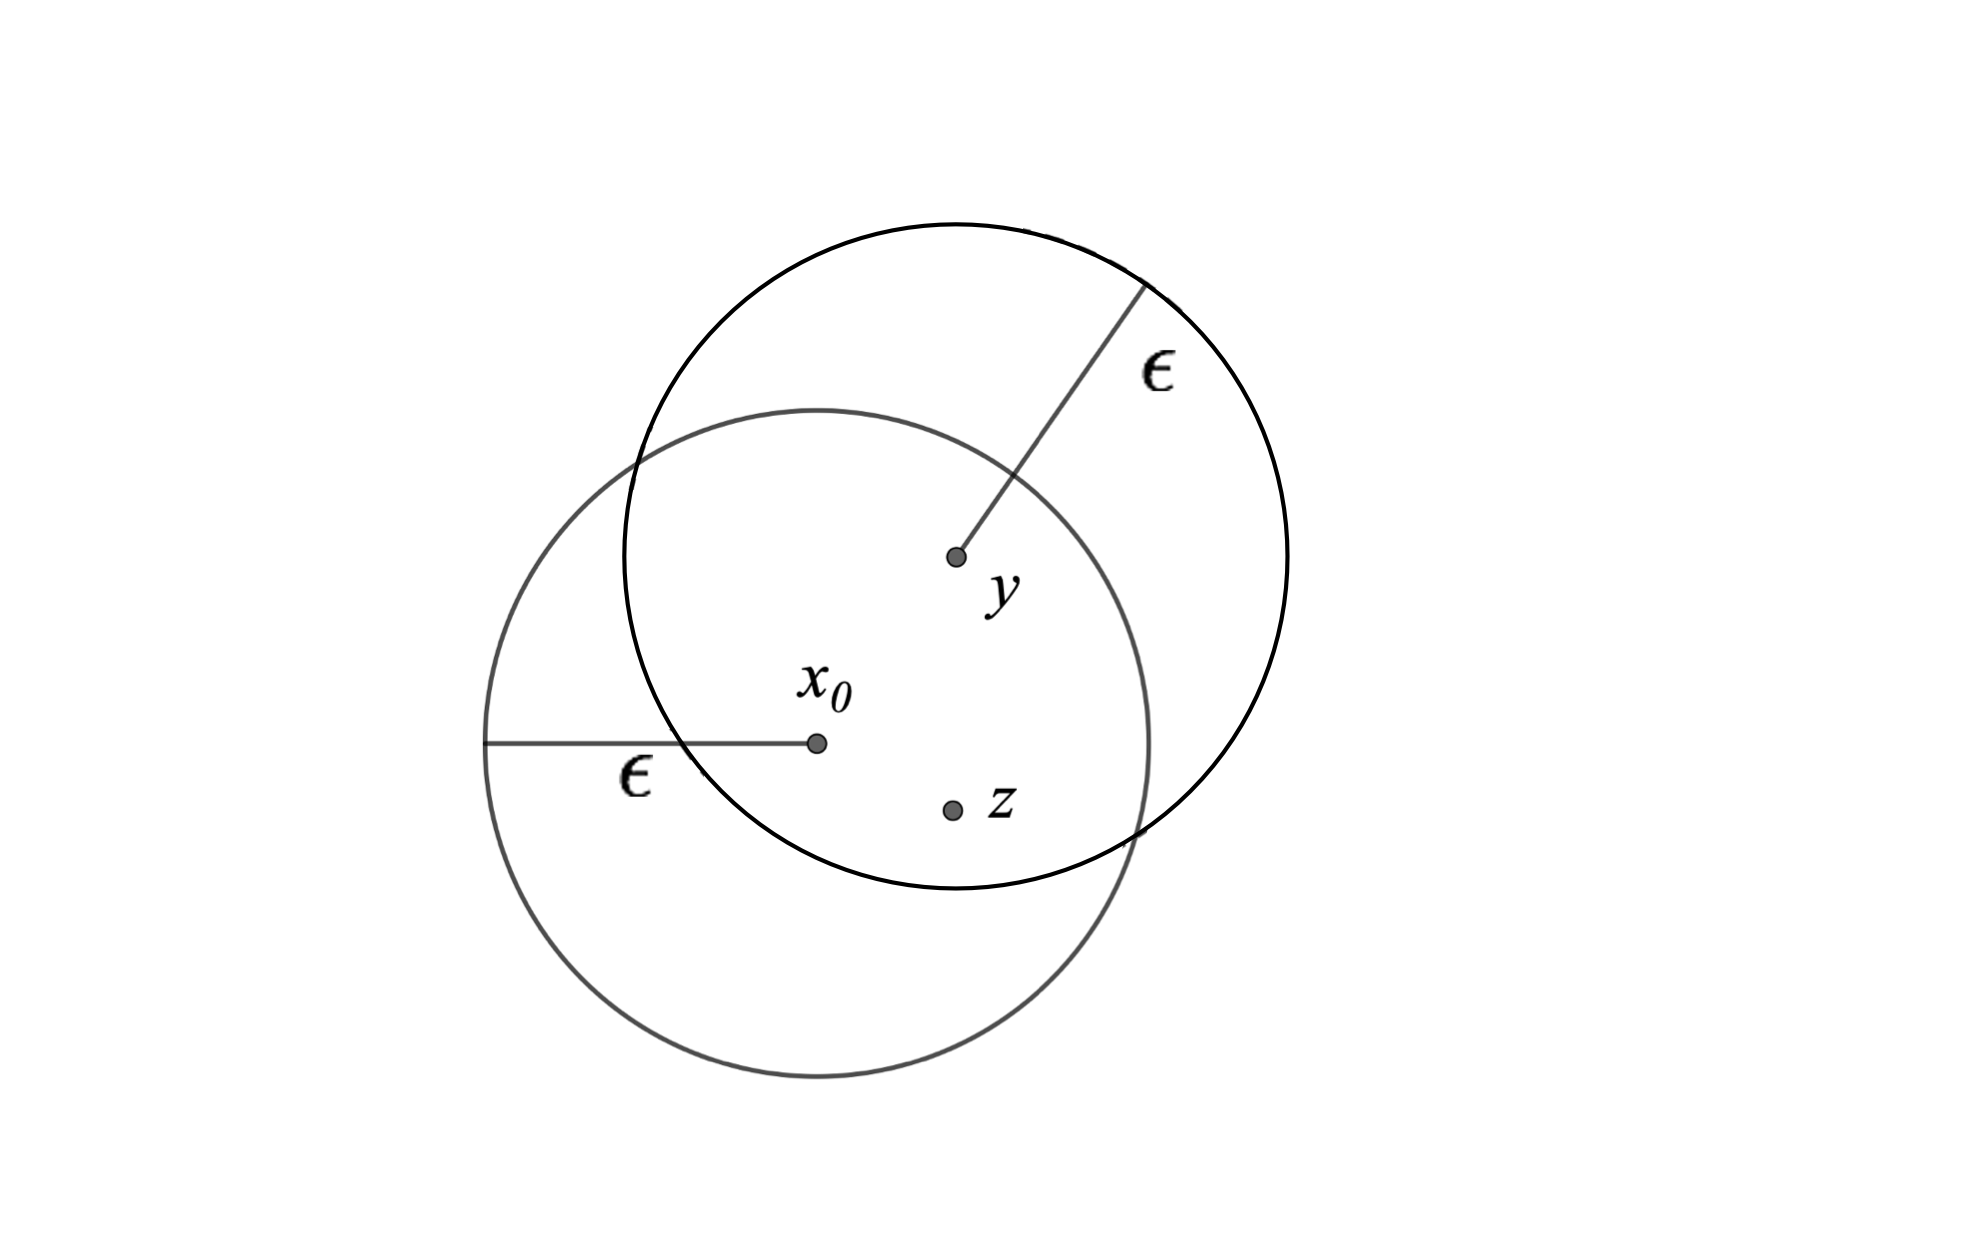
\includegraphics[scale=0.6]{necks_def.png}
	\end{frame}

	\begin{frame}{NEC\textit{k}Sc $\implies$ Multiple Minimum Spanning Trees}
		\begin{theorem} (From \cite{blevins_presentation}) \label{thm:necks_mmst}
			Let $(X, \dist)$ be a NEC\textit{k}S metric space for some $k \in \mathbb{N}$.
			Let $G(V, E)$ be the complete graph such that $V = X$ and for $(a, b) \in E$, $w(a, b) = \mrd(a, b)$.
			Then $G$ has multiple minimum spanning trees.
		\end{theorem}
		Dr. Blevins and Dr. Bridges showed this for NEC\textit{k}S spaces, but it also holds for NEC\textit{k}Sc spaces.
		So we need only to show that a data set (along with a definition of distance) is a NEC\textit{k}Sc metric space to show that it has multiple minimum spanning trees.
	\end{frame}

	\begin{frame}{Sufficient $k$ value}
		\begin{theorem}\label{thm:2d_k}
			For $k \geq 6$, \textit{any} two dimensional data set, with the $\ell^2$ norm as distance, is a NEC\textit{k}Sc space, and thus has multiple minimum spanning trees.	
		\end{theorem}
	\end{frame}

	\begin{frame}{Proof Sketch}
		Increasing $k$ cannot decrease $\epsilon$, so proving the theorem for $k = 6$ is sufficient to show it's truth for all $k \geq 6$.
		\begin{itemize}
			\pause
			\item Assume BWOC there exists some two-dimensional data set $X$ that is not a NEC\textit{k}Sc metric space for $k=6$ (with standard euclidian distance).
			\pause
			\item Order the six closest points to $x_0$ in terms of their angle relative to $x_0$.
			\pause
			\item By the definition of $\core_6(x_0) = \epsilon$, these are all within $\epsilon$ of $x_0$.
			\pause
			\item No pair of these points is within $\epsilon$ of each other, becuase $X$ is not a NEC\textit{k}Sc space.
		\end{itemize}
	\end{frame}

	\begin{frame}{Proof Sketch (continued)}
		\begin{itemize}
			\item This means that blue lines are strictly greater than $\epsilon$, and red/green lines are less than or equal to $\epsilon$.
			\pause
			\item The angles formed around $x_0$ sum to more than $2 \pi$.
			\pause
		\end{itemize}
		\center
		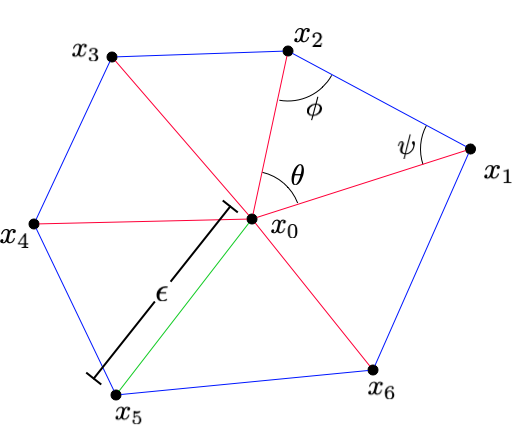
\includegraphics[scale=0.35]{2d_proof_fig.png}
	\end{frame}

	\section{Higher Dimensions}
	
	\begin{frame}{The Kissing Number}
		\begin{definition}\label{def:kissing_number}
			Given an $n$-dimensional sphere $S$ with radius $r$, the \textbf{$n$-dimensional kissing number} $\kiss(n)$ is the maximum number of spheres of radius $r$ that can be tangent to $S$ without the interiors of any two spheres overlapping*.
			
		\end{definition}
		*Two spheres' interiors overlap if their intersection is neither the empty set nor a single point.
	\end{frame}

	\begin{frame}{Background on the Kissing Number}
		% The kissing problem asks how many spheres can be arranged tangent to a given sphere, if they all have the same size and their interiors cannot overlap \cite{kissing_numbers}.
		Already hard in three dimensions: Newton disagreed with David Gregory about $\kiss(3)$.
		"Extra" space in 3D unlike in 2D.
		\vspace{0.2in}

		\center		
		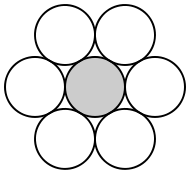
\includegraphics[scale=0.5]{1dkn.png}
		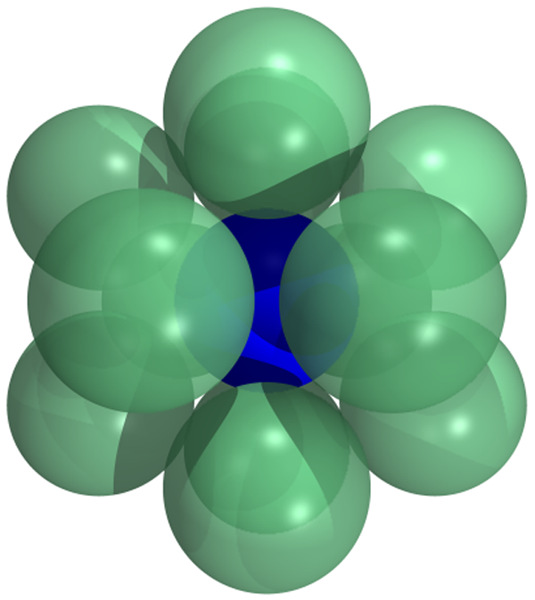
\includegraphics[scale=0.2]{kissing_picture.jpg}
	\end{frame}
	
	\begin{frame}{Kissing Numbers (from \cite{kissing_numbers})}
		\center
		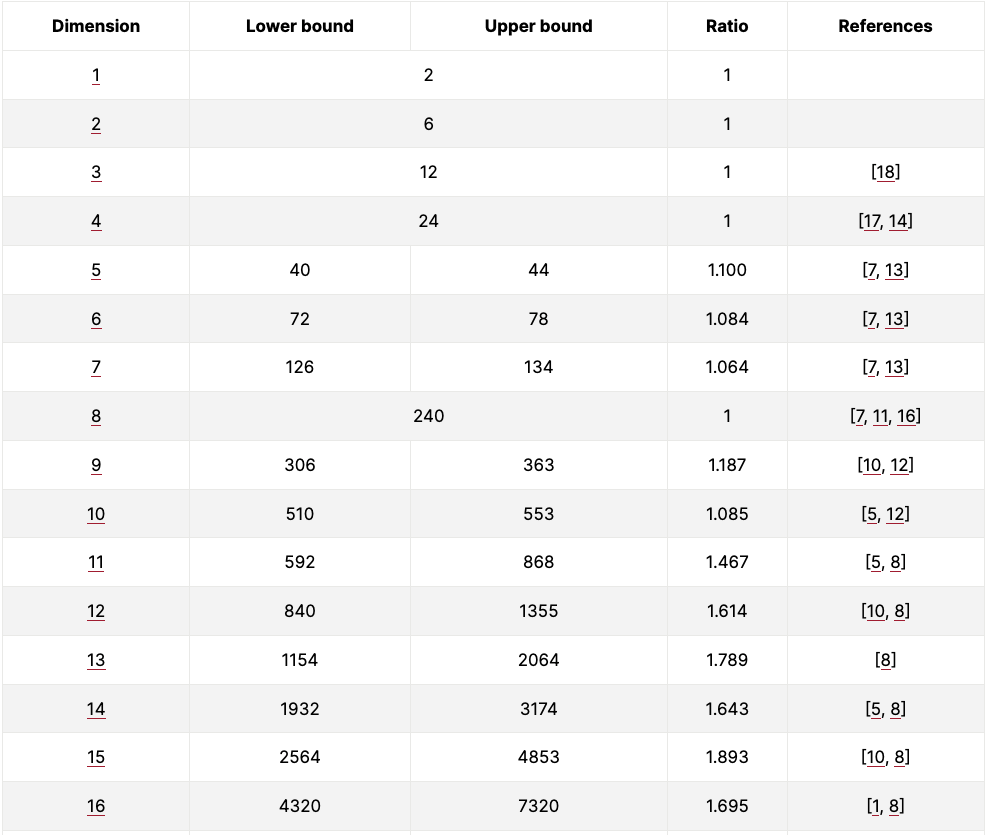
\includegraphics[scale=0.3]{kissing_nums_list.png}
	\end{frame}

	\begin{frame}{$k > \kiss(n) \implies$ NEC\textit{k}Sc}\label{thm:kiss_necksc}
		\begin{theorem}
			Let $X$ be n-dimensional data set, and let $\dist$ be euclidian distance.
			Then $(X, \dist)$ is a NEC\textit{k}Sc space if
			\begin{enumerate}
				\item $k > \kiss(n)$ and
				\item $|X| > k$*
			\end{enumerate}
		\end{theorem}
		*This second point is formally necessary but practically meaningless:
		$|X| \leq k$ would mean the data is all in one cluster.
	\end{frame}

	\begin{frame}{Proof Sketch}
		% Only need to show for $k = \kiss(n) + 1$, which will imply the result for all larger $k$.
		Let $X$ be an $n$-dimensional data set, and let $(X, \dist)$ \textbf{not} be a NEC\textit{k}Sc space.
		We show that this implies $k \leq \kiss(n)$.
		\begin{itemize}
			% \pause
			% \item Assume BWOC that there exists $n$-dimensional data set $X$ ($|X| > k$) that is not a NEC\textit{k}Sc metric space for $k = \kiss(n) + 1$.
			\pause
			\item Consider the $k$ closest points to $x_0$, call this set $A$.
			\pause
			\item Notice that $|A| = k$.
			\pause
			\item Let each $p \in A$ correspond to a new $p'$, on $\overrightarrow{x_0 p}$, with $\dist(x_0, p') = \epsilon \geq \dist(x_0, p)$.
			(Call this set of new points $A'$).
			\pause
			\item $|A'| = |A| = k$.
			\pause
			\item For all $p, q \in A$ with $p \neq q$, $\dist(p, q) > \epsilon$, becuase $(X, \dist)$ is not a NEC\textit{k}Sc space.
			\pause
			\item Because new points travel outward along diverging lines, we also know $\dist(p', q') > \epsilon$
			for all $p', q' \in A'$ with $p' \neq q'$.
		\end{itemize}
	\end{frame}

	\begin{frame}{Proof Sketch (continued)}
		\begin{itemize}
			\item We place a hypersphere of radius $\frac{\epsilon}{2}$ centered at each $p' \in A'$, as well as one centered at $x_0$.			
			\pause
			\item These hyperspheres are all tangent to the hypersphere centered at $x_0$, because for each $p' \in A'$, $\dist(p', x_0) = \epsilon$.
			\pause
			\item But no hypersphere is tangent to any other, because $\dist(p', q') > \epsilon$ for all $p', q' \in A'$ with $p' \neq q'$.
			\pause
			\item These all have radius $\frac{\epsilon}{2}$, so $\kiss(n) \geq k$ by definition.
		\end{itemize}
	\end{frame}

	\begin{frame}{Proof Illustration in Two Dimensions}
		\center
		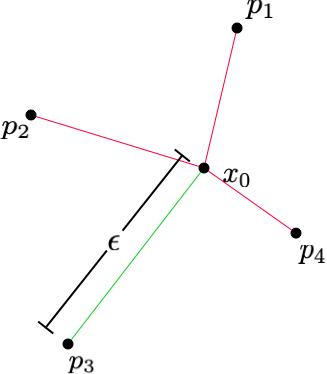
\includegraphics[scale=0.2]{kiss_proof_a.png}
		\pause
		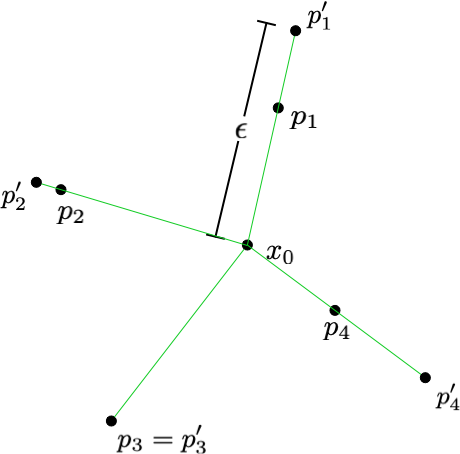
\includegraphics[scale=0.2]{kiss_proof_b.png}
		\pause
		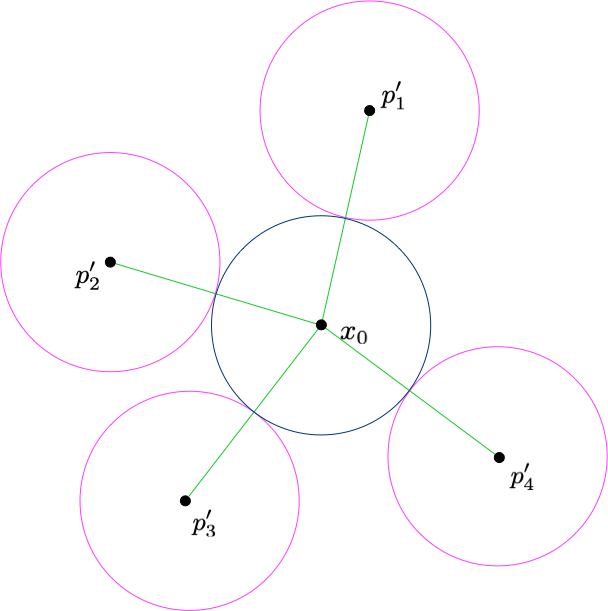
\includegraphics[scale=0.2]{kiss_proof_c.png}
	\end{frame}

	\section{Conclusion}

	\begin{frame}{Conclusion}
		\begin{itemize}
			\item We have verified that it is possible to get different minimum spanning trees from HDBSCAN over the same data set.
			\pause
			\item We have tested that this can occur in real-world data, and have empirically shown that this is often the case.
			\pause
			\item We have shown conditions that gurantee a metric space is NEC\textit{k}Sc, which imply non-unique minimum spanning trees.
		\end{itemize}
	\end{frame}
	
	\begin{frame}{References}
		\nocite{Unwin2021TheID}
		\nocite{hdbscan_tutorial}
		\nocite{blevins_presentation}
		\nocite{hdbscan_paper}
		\nocite{mnist}
		\nocite{kissing_numbers}
		\tiny
		\bibliographystyle{plain}
		\bibliography{refs} 
	\end{frame}

	\begin{frame}{Sports Come Up in a Data Clustering Presentation (Again)}
		\center
		
\includegraphics[scale=0.22]{kzx_superbowl_party.png}
	\end{frame}
\end{document}
